\documentclass{sigchi}

% Use this section to set the ACM copyright statement (e.g. for
% preprints).  Consult the conference website for the camera-ready
% copyright statement.

% Copyright
\CopyrightYear{2020}
%\setcopyright{acmcopyright}
\setcopyright{acmlicensed}
%\setcopyright{rightsretained}
%\setcopyright{usgov}
%\setcopyright{usgovmixed}
%\setcopyright{cagov}
%\setcopyright{cagovmixed}
% DOI
\doi{https://doi.org/10.1145/3313831.XXXXXXX}
% ISBN
\isbn{978-1-4503-6708-0/20/04}
%Conference
\conferenceinfo{CHI'20,}{April  25--30, 2020, Honolulu, HI, USA}
%Price
\acmPrice{\$15.00}

% Use this command to override the default ACM copyright statement
% (e.g. for preprints).  Consult the conference website for the
% camera-ready copyright statement.

%% HOW TO OVERRIDE THE DEFAULT COPYRIGHT STRIP --
%% Please note you need to make sure the copy for your specific
%% license is used here!
% \toappear{
% Permission to make digital or hard copies of all or part of this work
% for personal or classroom use is granted without fee provided that
% copies are not made or distributed for profit or commercial advantage
% and that copies bear this notice and the full citation on the first
% page. Copyrights for components of this work owned by others than ACM
% must be honored. Abstracting with credit is permitted. To copy
% otherwise, or republish, to post on servers or to redistribute to
% lists, requires prior specific permission and/or a fee. Request
% permissions from \href{mailto:Permissions@acm.org}{Permissions@acm.org}. \\
% \emph{CHI '16},  May 07--12, 2016, San Jose, CA, USA \\
% ACM xxx-x-xxxx-xxxx-x/xx/xx\ldots \$15.00 \\
% DOI: \url{http://dx.doi.org/xx.xxxx/xxxxxxx.xxxxxxx}
% }

% Arabic page numbers for submission.  Remove this line to eliminate
% page numbers for the camera ready copy
% \pagenumbering{arabic}

% Load basic packages
\usepackage{balance}       % to better equalize the last page
\usepackage{graphics}      % for EPS, load graphicx instead 
\usepackage[T1]{fontenc}   % for umlauts and other diaeresis
\usepackage{txfonts}
\usepackage{mathptmx}
\usepackage[pdflang={en-US},pdftex]{hyperref}
\usepackage{color}
\usepackage{booktabs}
\usepackage{textcomp}
\usepackage{colortbl}

% Some optional stuff you might like/need.
\usepackage{microtype}        % Improved Tracking and Kerning
% \usepackage[all]{hypcap}    % Fixes bug in hyperref caption linking
\usepackage{ccicons}          % Cite your images correctly!
% \usepackage[utf8]{inputenc} % for a UTF8 editor only

% If you want to use todo notes, marginpars etc. during creation of
% your draft document, you have to enable the "chi_draft" option for
% the document class. To do this, change the very first line to:
% "\documentclass[chi_draft]{sigchi}". You can then place todo notes
% by using the "\todo{...}"  command. Make sure to disable the draft
% option again before submitting your final document.
\usepackage{todonotes}


% ADDED FOR TABLES; NOT PART OF DEFAULT
\usepackage{makecell}

% Paper metadata (use plain text, for PDF inclusion and later
% re-using, if desired).  Use \emtpyauthor when submitting for review
% so you remain anonymous.
\def\plaintitle{Plexus: Guiding Novice Transport Planners through Expert-authored Data Stories}
\def\plainauthor{Allyza Mae Acu\~na, Krizia Lynn Chiu, Louise Anne Cortez, Sophia Therese Rivera, Rafael Cabredo, Briane Paul Samson}
\def\emptyauthor{}
\def\plainkeywords{Transport planning; Spatial analysis and interpretation; novice transport planners;co-design}
\def\plaingeneralterms{Documentation, Standardization}

% llt: Define a global style for URLs, rather that the default one
\makeatletter
\def\url@leostyle{%
  \@ifundefined{selectfont}{
    \def\UrlFont{\sf}
  }{
    \def\UrlFont{\small\bf\ttfamily}
  }}
\makeatother
\urlstyle{leo}

% To make various LaTeX processors do the right thing with page size.
\def\pprw{8.5in}
\def\pprh{11in}
\special{papersize=\pprw,\pprh}
\setlength{\paperwidth}{\pprw}
\setlength{\paperheight}{\pprh}
\setlength{\pdfpagewidth}{\pprw}
\setlength{\pdfpageheight}{\pprh}

% Make sure hyperref comes last of your loaded packages, to give it a
% fighting chance of not being over-written, since its job is to
% redefine many LaTeX commands.
\definecolor{linkColor}{RGB}{6,125,233}
\hypersetup{%
  pdftitle={\plaintitle},
% Use \plainauthor for final version.
%  pdfauthor={\plainauthor},
  pdfauthor={\emptyauthor},
  pdfkeywords={\plainkeywords},
  pdfdisplaydoctitle=true, % For Accessibility
  bookmarksnumbered,
  pdfstartview={FitH},
  colorlinks,
  citecolor=black,
  filecolor=black,
  linkcolor=black,
  urlcolor=linkColor,
  breaklinks=true,
  hypertexnames=false
}

% create a shortcut to typeset table headings
% \newcommand\tabhead[1]{\small\textbf{#1}}

% End of preamble. Here it comes the document.
\begin{document}

\title{\plaintitle}

\numberofauthors{6}
\author{
%   \alignauthor{Allyza Mae Acu\~na\\
%     \affaddr{De La Salle University}\\
%     \affaddr{Manila, Philippines}\\
%     \email{allyza\_acuna@dlsu.edu.ph}}\\
%   \alignauthor{Krizia Lynn Chiu\\
%     \affaddr{De La Salle University}\\
%     \affaddr{Manila, Philippines}\\
%     \email{krizia\_chiu@dlsu.edu.ph}}\\
%   \alignauthor{Louise Anne Cortez\\
%     \affaddr{De La Salle University}\\
%     \affaddr{Manila, Philippines}\\
%     \email{louise\_cortez@dlsu.edu.ph}}\\
% \alignauthor{Sophia Therese Rivera\\
%     \affaddr{De La Salle University}\\
%     \affaddr{Manila, Philippines}\\
%     \email{sophia\_rivera@dlsu.edu.ph}}\\
% \alignauthor{Rafael A. Cabredo\\
%     \affaddr{De La Salle University}\\
%     \affaddr{Manila, Philippines}\\
%     \email{rafael.cabredo@dlsu.edu.ph}}\\
% \alignauthor{Briane Paul V. Samson\\
%     \affaddr{Future University Hakodate}\\
%     \affaddr{Hakodate, Japan}\\
%     \affaddr{De La Salle University}\\
%     \affaddr{Manila, Philippines}\\
%     \email{briane.samson@dlsu.edu.ph}}\\
  \alignauthor{Leave Authors Anonymous\\
    \affaddr{for Submission}\\
    \affaddr{City, Country}\\
    \email{e-mail address}}\\
  \alignauthor{Leave Authors Anonymous\\
    \affaddr{for Submission}\\
    \affaddr{City, Country}\\
    \email{e-mail address}}\\
  \alignauthor{Leave Authors Anonymous\\
    \affaddr{for Submission}\\
    \affaddr{City, Country}\\
    \email{e-mail address}}\\
  \alignauthor{Leave Authors Anonymous\\
    \affaddr{for Submission}\\
    \affaddr{City, Country}\\
    \email{e-mail address}}\\
  \alignauthor{Leave Authors Anonymous\\
    \affaddr{for Submission}\\
    \affaddr{City, Country}\\
    \email{e-mail address}}\\
  \alignauthor{Leave Authors Anonymous\\
    \affaddr{for Submission}\\
    \affaddr{City, Country}\\
    \affaddr{for Submission}\\
    \affaddr{City, Country}\\
    \email{e-mail address}}\\
}
\maketitle

\begin{abstract}
  Transport planning enables governments to ensure sustainable mobility in cities. Often done by a national agency, some countries decentralize this to local governments with mostly novice planners and non-expert teams. This can be counterproductive because they lack expertise in collecting, analyzing and synthesizing transport-related data for sound policy-making. Current tools can be too complicated for novice planners especially with evolving assessment frameworks, requiring expert knowledge and training. Through co-design, we identified the workflow patterns of transport engineers and mental models of novices, and iteratively developed Plexus, a web application designed to support transport desirability assessment using expert-authored data stories. We found that the use of expert-authored data stories with traditional exploratory tools put novice planners in the proper mindset and improved the way they assessed transport desirability while reducing their mental workload.
\end{abstract}


% ACM Classfication

 \begin{CCSXML}
<ccs2012>
<concept>
<concept_id>10003120.10003123.10010860.10010859</concept_id>
<concept_desc>Human-centered computing~User centered design</concept_desc>
<concept_significance>500</concept_significance>
</concept>
</ccs2012>
\end{CCSXML}

\ccsdesc[500]{Human-centered computing~User centered design}
\ccsdesc[500]{Human-centered computing~Human computer interaction (HCI)}
\ccsdesc[100]{Human-centered computing~User studies}

% Author Keywords
\keywords{\plainkeywords}

% Print the classficiation codes
\printccsdesc
% Please use the 2012 Classifiers and see this link to embed them in the text: \url{https://dl.acm.org/ccs/ccs_flat.cfm}



\section{Introduction}

Transport planning is a collaborative process that requires the involvement of stakeholders to strategize on the operation, maintenance, and management of a place\'s transportation system to meet their long-term transportation and mobility goals. It can ease the effects of urbanization by helping stakeholders understand a place\'s geography and finding strategic solutions for its underlying mobility challenges \cite{Palma2017}, ranging from environmental impacts to equity and accessibility. Because of its dynamic nature, transport planning has become a complex analytical and cyclical process of balancing multiple decision criteria from a range of factors \cite{Simao2009}.

Formal and expert knowledge on transport engineering and experience in transportation planning tools are ideal to make data-driven assessments and plans on building infrastructure, zoning, and route planning. However, the lack of transport planning education has caused developing countries to barely endure rapid urbanization \cite{evren2001transportation}. Additionally, the lack of integrated planning across transport modes and land use, conflicting government policies at local and national levels, misaligned plans, and lack of funds have led  to developing countries having poor transport infrastructure \cite{mahendra2016,gwilliam1999public}. In the context of the Philippines, there is an imbalance in the development of urban planning divisions between local government units (LGUs). Although a comprehensive land-use plan (CLUP) is currently utilized by Philippine cities and municipalities, departments officials for transport planning or transport management are not required to have formal training in such. Moreover, officials are also not required to have knowledge in systems that aid in transport planning, as most government units cannot afford to acquire such systems.  

Due to this, there is a challenge when making transport-related decisions for officials since they are tasked to create assessments for transportation problems. As compared to experts who are formally trained in transport engineering and have learned concepts and theories regarding these, government officials lack the knowledge, training, and resources such as analysis tools to formulate assessments that are as data-driven. However, these tools only provide features for users to decide on relevant information for them, and not necessarily guiding them to create an assessment. Some examples of tools that are utilized for transport planning are QGIS, EMME, Cube, JICA Strada, and Visum, but are more catered to experts. The usage of these tools often relate to travel demand forecasting models, cost-benefit analysis, statistical graphs, and simulations, and are utilized in modeling traffic or transport patterns. Multiple visualizations for statistical analysis and other supporting data superimposed on map visualizations, as well as the capacity to view raw data in a table view are also present in these systems. However, since the user is given the freedom of choosing visualizations for various data, it can overwhelm novices, leading to the inability to maximize the insights they could gather.Therefore, the ideal process and quality of assessment experts have may be difficult for novices to achieve.

Transport desirability is a new transport assessment framework which shows how desirable an area is based on accessibility, travel data, and commuter experiences. Although this framework will be used by LGU planners in the future, its complexity may hinder LGU planners, who are novices, to create quality assessments. In this study, we designed a novice support tool, Plexus, which is a middle ground between the standard practice of the engineers and the mental models of novices. Since novice planners lack the experience, knowledge, and resources in formulating transport assessments, co-design sessions served as avenues for both novice and expert planners to discuss needed information and visualizations for transport desirability assessment.  By establishing the workflow, interface, interactions, and features, we implemented the tool and iteratively consulted with novices and experts through usability tests to refine the features for Plexus. The final prototype is an exploratory tool that consists of an interactive map and data stories, which guides novices to create a transport desirability assessment with less difficulty.

In order to test if our hypothesis was true, we conducted a controlled study wherein we divided our users into three groups, each having three novice planners. The users were asked to formulate transport assessments using (a) spreadsheet applications, (b) Plexus without the data stories, and (c) Plexus with data stories. We utilized a task-based test and asked the participants to evaluate their workload using NASA-TLX, as well as give transport assessments using their assigned tools. 

\section{Related Work}

\subsection{Novice Support Tools}
Novice support tools have simplified interfaces and limited functions to lessen the cognitive load of users. These tools are created to make difficult tasks, usually requiring expert knowledge, easier for novices. Moreover, these  tools are created to ease the difficulty of learning a skill or a process. DrawMyPhoto is an example of a tool that focused on simplifying interfaces by removing grids and limited functions by removing manually chosen stroke width, color, and darkness \cite{Williford2019}. The system also adopts techniques from experts by using light blue color for reference images, which is a popular underlay color in architectural drafting. Motif is another tool that supports novices to create expert-like outputs using expert patterns that novices need to follow \cite{Kim2015}. Other than these studies, other related studies are evaluated through an expert assessing the outputs of novices. In the case of both Motif and DrawMyPhoto, the studies achieved positive results in supporting novices with achieving difficult tasks.  

\subsection{Data Stories}
Data stories are a combination of narratives and interactive or static data visualizations \cite{Segel2011}. Usually, data visualizations provide supporting or related details to the narrative. Narratives are presented in a meaningful order to communicate ideas from the author to the readers, which can be called author-driven \cite{Lee2015}. However, the arrangement of these narratives could also be reader-driven, wherein there is no strict order of information and a high degree of interactivity \cite{Segel2011}. Choosing between these two approaches depends on the complexity of the data and narrative, and the intended audience. Utilizing messaging to explain ideas and data visualizations may clarify the narrative, but might clutter the interface. On the other hand, interactivity may engage user exploration, but might not lead to the intended message of the author. 

There has been an ongoing discussion about data stories being beneficial. Multiple studies have concluded that data stories were seen as a powerful way to summarize various information, to subtly explore data, to discover new questions about the data, and to deliver ideas or messages to the readers \cite{Pavel2013} \cite{Layton2014}. FinaVistory used data stories to help readers understand financial news \cite{Chan2016}; However, the data stories were interactive, allowing users to choose what to focus on. In MeetingVis, data stories were effective in memory retrieval for meetings through showing essential meeting elements \cite{Shi2018}. Other than interactivity, tooltips and backstories to clarify context were considered beneficial by Figueiras \cite{Figueiras2014}. This is supported in the study of GameFlow, which stated that although users were satisfied with the visualizations, textual narrations to complement the visualizations were suggested \cite{Chen2016}. Although these studies curated data stories, stakeholder participation in design and in evaluation was not prioritized. Moreover, evaluation was feature-based and not focused on the effect on understanding messages. Therefore, our study aims to contribute by incorporating co-design in creating the application and evaluation of resulting assessments through data stories. 

\section{Co-design of Plexus}

To ensure the effectiveness of a tool being developed, studies posit that involving end-users and consultants early on in the design process is a beneficial step. Co-design supports discussion with end-users, consultants, and  proponents regarding the design of the interface, features, and workflow of the tool. The process of co-design considers the end-users\' everyday work practices and offers a goal for learning for practitioners  (\cite{roschelle:2006}). For SpeechBubbles, multiple interviews were done with end-users to understand their situation and pain points. After analyzing the pain points of the participants, they were asked to design visualizations and suggest features with other participants. Insights from the session led to the creation of the prototype, which was refined through multiple design critiques with co-design participants. In a different study, \cite{mazzone:2011}  proposed to simplify a co-design framework when designing a session for children, as the process, while complex, is important when adult designers are creating a tool for a child\'s mental model.  A who-what-when-where-how (WH/HW) framework was utilized, which considers the consultation of experts in validating activities during co-design since their insights are beneficial when designing for novices.

In \cite{roschelle:2006}, the integration of innovative learning techniques such as software tools in classroom settings were tested through a co-design with teachers, who underwent a series of interviews and rapid prototyping. They were able to utilize the prototypes of the tools with the students, and were able to engage in the process of modifying their current practices through a systematic approach. \cite{Alhumaidan2015} used co-design on low-tech prototyping, and involved groups of children, teachers, and HCI experts. Using co-design reveals the challenges faced by each stakeholder, which leads to proponents adjusting workflow, interface, and features in the tool as early as possible. 

In order to develop Plexus for novice transport planners, we conducted two co-design sessions. The participants involved were expert planners and LGU officials in order to obtain and validate insights from multiple perspectives regarding transport planning and the implementation of Plexus. The goal of the co-design approach is to gather information from various stakeholders about the transport planning workflow and types of information that will be presented in the system. Through this, we would be able to model Plexus in a way that is familiar to transport planners.

For the first co-design session, three activities were done. We first asked participants to elaborate their current step-by-step transport planning process through journey mapping as seen in Figure \ref{fig:codesign2}, which tasked them to write and discuss the action, data visualization and tool, and thought process or questions for each step. Participants were also asked to identify which steps in the process of other planners they consider as good practices. Through this, it is easier to identify similarities and differences in the transport planning processes of different participants, as well as get a consensus of what counts as a notable planning practice. From this, affinity diagrams were created to determine pain points in these processes. We did this by asking each participant to write down questions they have about transport planning, but do not have the answer to due to the lack of resources or capabilities available to them. Finding the types of information that would answer these questions were done through card sorting. For this activity, a set of cards containing containing visualization techniques, indicators, or qualities provided by the transport desirability framework were given to the participants. While working either individually or in groups, participants were asked to associate them with the categorized issues from the affinity diagram.

The second co-design session focused on identifying explanatory data for each indicator in the transport desirability framework through the use of card sorting. Compared to the first session, only two experts were asked to relate visualizations and data, as well as their order of presentation, for the different indicators. This was done to aid us in organizing the information to be shown in the system in a way that would be easily understood by novice planners.

\subsection{First co-design session: Understanding Planning Practices}

\begin{figure}
\centering
  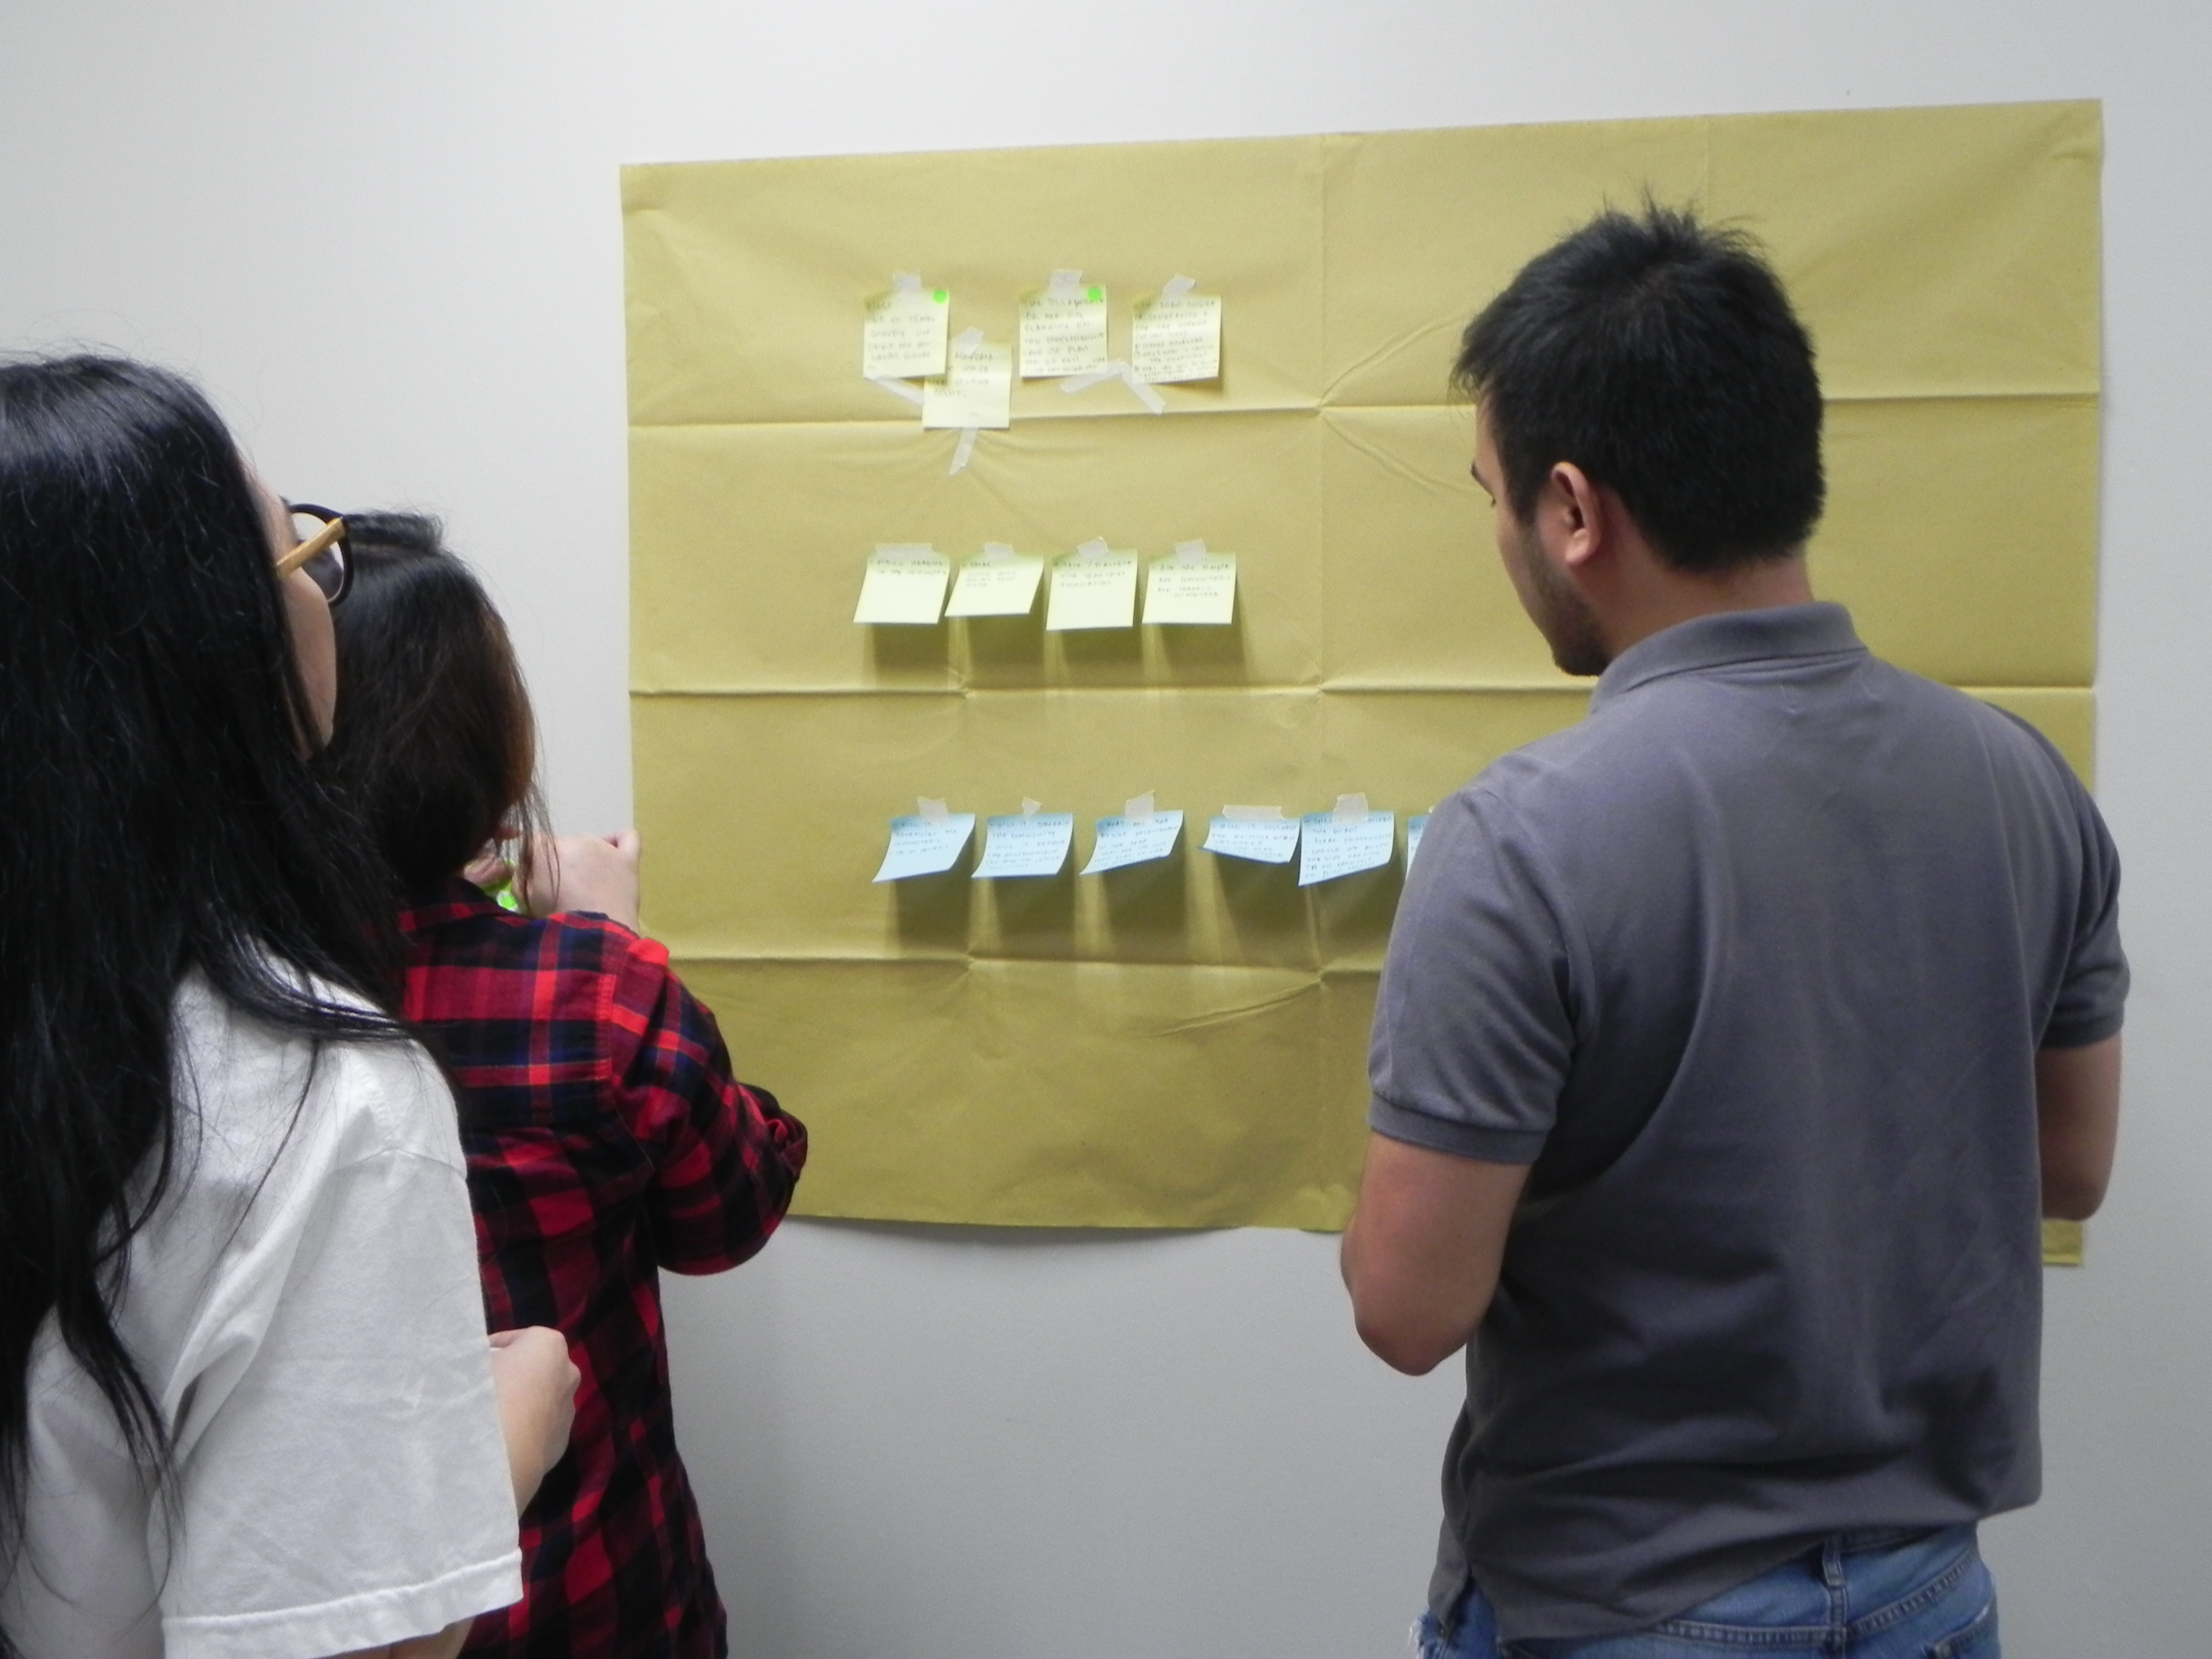
\includegraphics[width=0.8\columnwidth]{figures/photos/DSCN9673.JPG}
  \caption{Transport planner using journey mapping to explain their current process}~\label{fig:codesign2}
\end{figure}

The initial session aimed to identify the current state of transport planning for both novice and expert planners, as well as their expectations when creating transport assessments. Since there is a difference between the transport planning processes of the participants, the session allowed them to explore various practices and ultimately collaborate on an information architecture for Plexus. Findings from this session consist of the expected data and visualizations to be presented to the participants, and how they will navigate the system when making an assessment. This session had four local government officials under the department of planning or transport management [G1-G4] and 1 subject-matter expert [S1] who was a transport engineer. 

\subsection{Insights}
\subsubsection{Strategies for decision-making are trial-and-error}
From the co-design session, an eminent theme was the insufficiency of data and resources for transport planning. Varying processes in transport planning have elicited different results from LGUs with regard to their process. However, officials from both cities base their decisions on observations or assumptions of the current traffic situation and socioeconomic and vehicle count data. These decisions, however, are evaluated based on the degree of traffic congestion observed in the area and are not based on commuter opinions or recorded data. 

\subsubsection{Tools to aid in transport planning are not used or are difficult to use}
Aside from the lack of a centralized process, all LGU officials have mentioned that they do not use any tool to help them in their tasks, and instead rely on non-visualized data and observations of the area. Although they use maps for observing the land-use in the area, they do not use other visualizations besides choropleth maps. Additionally, according to S1, current systems such as EMME are difficult to use without prior training.  

\subsubsection{Most participants lack useful data and visualizations}
In line with this, data from commuters are significantly deficient as G3 and G4 have mentioned wanting to be knowledgeable about commuters\' opinions on changes in public transport. As officials do not have access to more information regarding transport and commuter behavior, the current process results to decisions in their city being tested through trial and error for G1, G3, and G4. Apart from this, accessible data is usually presented in figures and may not be aggregated.

Due to this issue, officials expect that they would make more informed transport decisions when given more and well-presented data. Data stated to be useful include origin and destination points, spatial amenities in the area, and economic and temporal indicators from the transport desirability framework. From this, they also mapped visualizations that they think would assist them in assessing transport in their respective cities. Choropleth maps were said to be understandable for representing indicators per barangay, lines and arcs were appropriate for origin and destination points and volume of commuters for a path, and icon maps were stated to be used to visualize amenities. Other visualizations such as hexagon binning and heatmaps were not utilized by the stakeholders.

\subsection{Second Co-design Session}
The second session was to identify data that would be beneficial in assessing each transport desirability indicator. This session had 2 transport desirability experts participate through cardsorting lists that were initially made using the first session insights. The cards consisted of the data, their visualizations, and the order of how this data will be presented to the user.

\subsection{Insights}
\subsubsection{General Information}
Demographic data, overall modeshare, and modeshare per barangay were deemed as important information and should be present when viewing any indicator or transport desirability. An indicator breakdown was also suggested to promote a top-down analysis. Land area, amenities, and origin-destination data were also considered as important information in assessing barangays, which are areas that are smaller than towns or cities. 

\subsubsection{Transport Desirability}
The co-design session resulted to three groups of information that LGUs believed would be useful to users. These groups are namely: 1) Route Development, 2) Mode Shift, and 3) Flooding. 

For information related to routes, origin-destination data along with their corresponding distances, travel costs, volume, and travel time, and mode share of the barangay was suggested by the experts. It would also be ideal for users to filter these information through demographics. Under Mode Shift, average comfort per transport mode, mode share by demographic, breaking down an origin-destination pair by mode share, health contribution per transport mode, travel time and travel cost per transport mode was suggested. Lastly, information that would be used to assess barangays and the city/town with regard to flooding were origin-destination pairs most affected by flood, survey results on how much a trip is affected by flood, range of travel cost and additional travel costs, range of travel time and additional travel time, energy use of transport mode, efficiency of per transport mode, and route and mode options during heavy rain and flooding. 

\subsubsection{Indicators}
Economic and temporal indicators would require the average, maximum, and minimum travel cost and travel time, top 10 and bottom 10 travel cost and travel time, cost and time to and from one barangay to another for public and private transport mode, mode share, amenities, and income distribution to assess properly. Data suggested for deeper assessment of the physical indicator would be the effect on commuters in terms of the percentage of people who are flooded along with their origin-destination pair, average, maximum, and minimum cost of commuters with their origin-destination pairs. A link to amenities and the answers to flood-related survey questions presented as a bar graph were also deemed useful. For the spatial indicator, it would be beneficial to present the accessibility of different income levels depending on their travel allowance, a breakdown count of per amenity, and a list of amenities that are reachable from a certain distance or time. For transport mode indicators, each would be linked to the physical indicator and spatial indicator as they were deemed useful.

\section{Designing Plexus}
Plexus is a visual analytics system that aims to aid novice users attain expert-like transport desirability assessments through interactive elements and data stories. 

% Specifically, the system allows users to view and visualize cities\' and barangays\' transport desirability and transport desirability-related factors. It first directs the user to the home screen, where the list of available cities are presented to the user. Upon selecting a city from the Plexus home screen, the user would be directed to the assessment screen, containing various interactive elements: the map, the left side panel containing the city overview, the right side panel containing indicator overviews or barangay overviews, and the collapsed bottom panel containing data stories. Through the combined use of these various elements, the users could be aided with the transport assessment of the city.

We conducted 4 usability tests to refine the feautres, flow, and interface. All usability tests had task-based evaluation with tasks on assessing the city, its barangays, and barangay comparisons. After each task, participants had to answer the NASA-TLX questionnaire. The last 3 usability tests tasked participants to explore Plexus before proceeding with the tasks, while the last 2 usability tests had a guide for participants to uunderstand transport desirability concepts. Table 1 shows the usability testing iterations done throughout the study:

% \begin{table*}[h!]
% \begin{tabular}{c{0.5cm} c{1cm} c{2cm}}
% \hline 
% Iteration & Goals & Participants\\ 
% \hline 
% UT1 & 
% \makecell{To get comments about the initial  implementation from novice and expert perspectives\\ \\To find a middle ground between all comments to drive system improvements} &
% \makecell{  \\ 3 Novices \\ (Metro Manila LGU officials, \\ Engineering student) \\ \[1UN1-3\]
% \\  \\ 3 Experts \\ (Transport engineer, \\ Transport Desirability experts) \\ \[1UE1-3\]}

% \\ 
% \hline 
% UT2 & 
% \makecell{To test on new novice users who are unfamiliar with the system\\
% \\To check how intuitive the system is after implementing suggestions from UT1 \\
% \\To find out from experts the quality of the novices\' assessments \\
% \\To get suggestions from experts on how to improve assessments\\
% } &
% \makecell{  \\ 6 Unfamiliar Novices \\ (Engineering students) \\ \[2UN1-6\]
% \\  \\ 3 Familiar Novices \\ (Metro Manila LGU officials,\\ Engineering student) \\ \[2FN1-3\]\\
%  \\ 2 Familiar Experts \\ (Transport Desirabilty Expert, \\ Transport Engineer) \\ \[2FE1-2\]} 
% \\ 
% \hline 
% UT3 & 
% \makecell{To test if the system would still be usable for other LGUs even if we co-designed\\ with only Metro Manila LGUs\\
% \\
% To test if expounded descriptions would have a positive effect\\ on mental workload and confidence\\
% } &
% \makecell{  \\ 3 Unfamiliar Novices\\ (Provincial LGU officials)\\ \[3UN1-3\]} 
%  \\
% \hline
% UT4 & 
% \makecell{To check the usability of the system for experts \\who are unfamiliar with the system\\ \\
% To determine if the transport desirability framework concept may have affected \\the assessments of novices due to its complexity
% \\
% } &
% \makecell{  \\ 2 Unfamiliar Experts\\ (Transport Engineers)\\ \[4UN1-2\]} 
% \\ 
% \end{tabular} 
% \caption{Overview of the 4 usability tests done for this study as well as their corresponding goals and participants} \label{tab:ut}
% \end{table*}

\begin{table*}[!htbp]
\small
    \centering
    \begin{tabular}{p{0.052\textwidth}|p{0.6\textwidth}|p{0.3\textwidth}}
    \toprule
        \multicolumn{1}{c}{Iteration} & 
        \multicolumn{1}{c}{Goals} & 
        \multicolumn{1}{c}{Participants} \\
        \midrule
        UT1 & 
        \begin{itemize}
            \item To get comments about the initial implementation from novice and expert perspectives
            \item To find a middle ground between all comments to drive system improvements
        \end{itemize} 
        & \begin{itemize}
            \item 3 Novices - Metro Manila LGU officials, Engineering student (1UN1-3) 
            \item 3 Experts - Transport engineer, Transport Desirability experts (1UE1-3) 
        \end{itemize}\\ \hline
        
        UT2 &
        \begin{itemize}
            \item To test on new novice users who are unfamiliar with the system
            \item To check how intuitive the system is after implementing suggestions from UT1
            \item To find out from experts the quality of the novices' assessments
            \item To get suggestions from experts on how to improve assessments
        \end{itemize}
        & \begin{itemize}
            \item 6 Unfamiliar Novices - Engineering students (2UN1-6)
            \item 3 Familiar Novices - Metro Manila LGU officials, Engineering student - (2FN1-3)
            \item 2 Familiar Experts - Transport Desirabilty Expert, Transport Engineer (2FE1-2)
        \end{itemize} \\ \hline
        
        UT3 &
        \begin{itemize}
            \item To test if the system would still be usable for other LGUs even if we co-designed with only Metro Manila LGUs
            \item To test if expounded descriptions would have a positive effecton mental workload and confidence
        \end{itemize}
        & 3 Unfamiliar Novices - Provincial LGU officials (3UN1-3) \\
        \hline
        
        UT4 &
        \begin{itemize}
            \item To check the usability of the system for experts who are unfamiliar with the system
            \item To determine if the transport desirability framework concept may have affected the assessments of novices due to its complexity
        \end{itemize}
        & 2 Unfamiliar Experts - Transport Engineers (4UN1-2) \\
    \bottomrule
    \end{tabular}
    \caption{Overview of the 4 usability tests done for this study as well as their corresponding goals and participants}
    \label{tab:ut}
\end{table*}

% \begin{table*}
% \centering
% \caption{Overview of the 4 usability tests done for this study as well as their corresponding goals and participants}
% \label{tab:ut}
% \begin{tabular}{|p{1cm}|p{6cm}|p{3cm}|} 
% \cline{1-3}
% {UT1} & \begin{tabular}[c]{@{}l@{}}\begin{tabular}{@{\labelitemi\hspace{\dimexpr\labelsep+0.5\tabcolsep}}l}{To get comments about the initial implementation from novice and expert perspectives}\\{To find a middle ground between all comments to drive system improvements}\end{tabular}\end{tabular}& \begin{tabular}[c]{@{}l@{}}\begin{tabular}{@{\labelitemi\hspace{\dimexpr\labelsep+0.5\tabcolsep}}l}{3 Novices~}{(Metro Manila LGU officials, Engineering student)~}1UN1-3~\\{3 Experts (Transport engineer, Transport Desirability experts)~}1UE1-3\end{tabular}\end{tabular}  \\ 
% \cline{1-3}
% UT2 & \begin{tabular}[c]{@{}l@{}}\begin{tabular}{@{\labelitemi\hspace{\dimexpr\labelsep+0.5\tabcolsep}}l}{To test on new novice users who are unfamiliar with the system}\\{To check how intuitive the system is after implementing suggestions from UT1}\\{To find out from experts the quality of the novices\' assessments}\\{To get suggestions from experts on how to improve assessments}\end{tabular}\end{tabular} & \begin{tabular}[c]{@{}l@{}}\begin{tabular}{@{\labelitemi\hspace{\dimexpr\labelsep+0.5\tabcolsep}}l}{6 Unfamiliar Novices }{(Engineering students) }{2UN1-6}\\{3 Familiar Novices (Metro Manila LGU officials, Engineering student)~}{2FN1-3}\\{2 Familiar Experts (Transport Desirabilty Expert, Transport Engineer) }{2FE1-2}\end{tabular}\end{tabular} &   \\ 
% \cline{1-3}
% UT3 & \begin{tabular}[c]{@{}l@{}}\begin{tabular}{@{\labelitemi\hspace{\dimexpr\labelsep+0.5\tabcolsep}}l}{To test if the system would still be usable for other LGUs even if we co-designed with only Metro Manila LGUs}\\{To test if expounded descriptions would have a positive effecton mental workload and confidence}\end{tabular}\end{tabular} & {3 Unfamiliar Novices~}{(Provincial LGU officials)~}{3UN1-3} \\ 
% \cline{1-3}
% UT4 & \begin{tabular}[c]{@{}l@{}}\begin{tabular}{@{\labelitemi\hspace{\dimexpr\labelsep+0.5\tabcolsep}}l}{To check the usability of the system for experts who are unfamiliar with the system}\\{To determine if the transport desirability framework concept may have affected the assessments of novices due to its complexity}\end{tabular}\end{tabular}  & {2 Unfamiliar Experts~}{(Transport Engineers)~}{4UN1-2}  \\
% \cline{1-3}
% \end{tabular}
% \end{table*}
                                                                  
%We conducted four usability tests to refine system features and interface. The first usability test (UT1) included three novices from Metro Manila local government units (LGUs) who were part of the planning or transport management department and did not have any formal training in transport engineering and its tools (UT1N). Three experts (UT1E), who specialized in transport desirability assessment or transport engineering, were also included in the first usability test. The second usability test (UT2) included six novices who were knowledgeable in engineering concepts (UT2NN) and three novices who participated in the previous test (UT2FN). Two experts (UT2E) from the first usability test were invited again to participate in the second iteration. The third usability test (UT3) had three novices from Provincial local government units (UT3N) to test if the system would still be usable for them even if we co-designed with only Metro Manila LGUs. Finally, the fourth usability test (UT4) had two new experts (UT4E), who specialized in transport engineering, test the system to check the usability of the system for a trained eye.

From the insights of all usability tests, we designed a tool with the following features: 

\subsection{Exploring the Interactive Map}

% \begin{figure}
% \centering
%   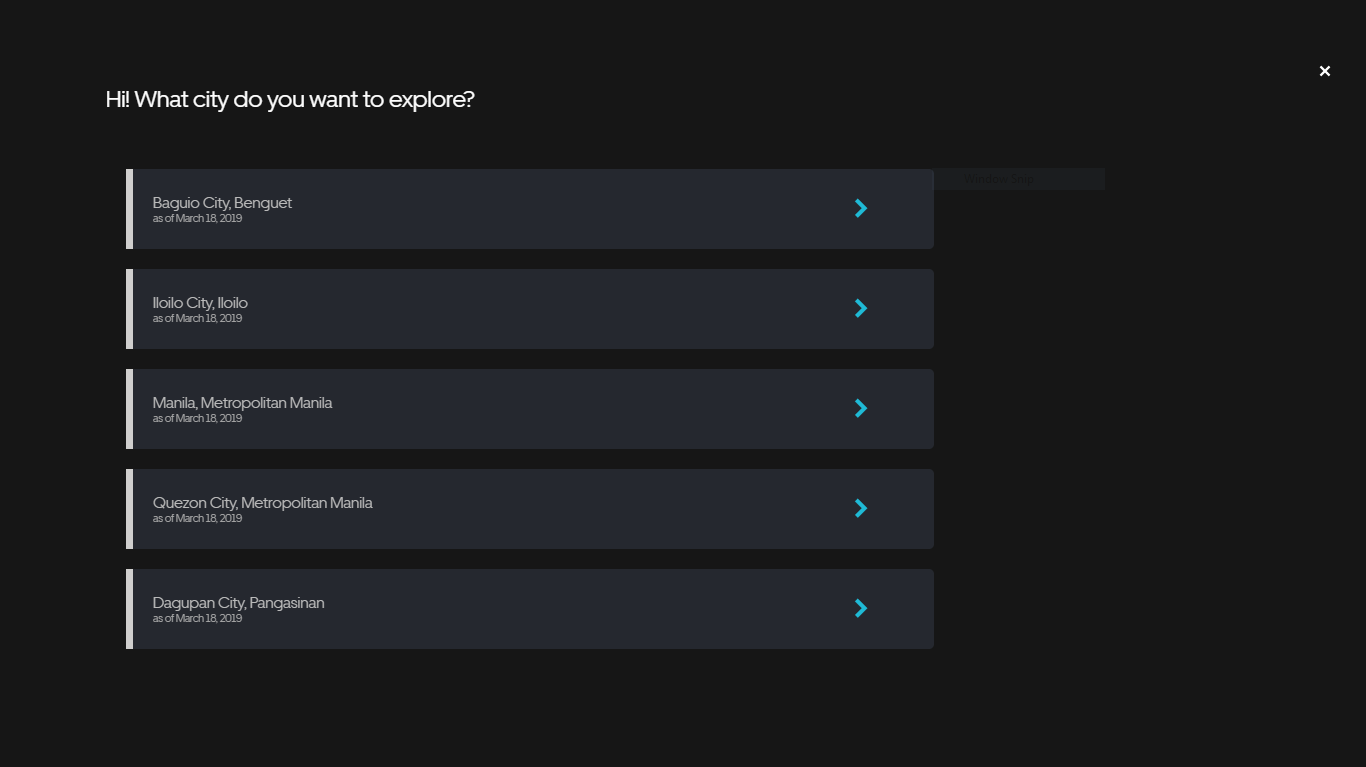
\includegraphics[width=0.9\columnwidth]{figures/kepler1.PNG}
%   \caption{Initial view of Plexus where a user can choose what to view from the list of published cities }~\label{fig:KeplerCityList}
% \end{figure}

\begin{figure}
\centering
  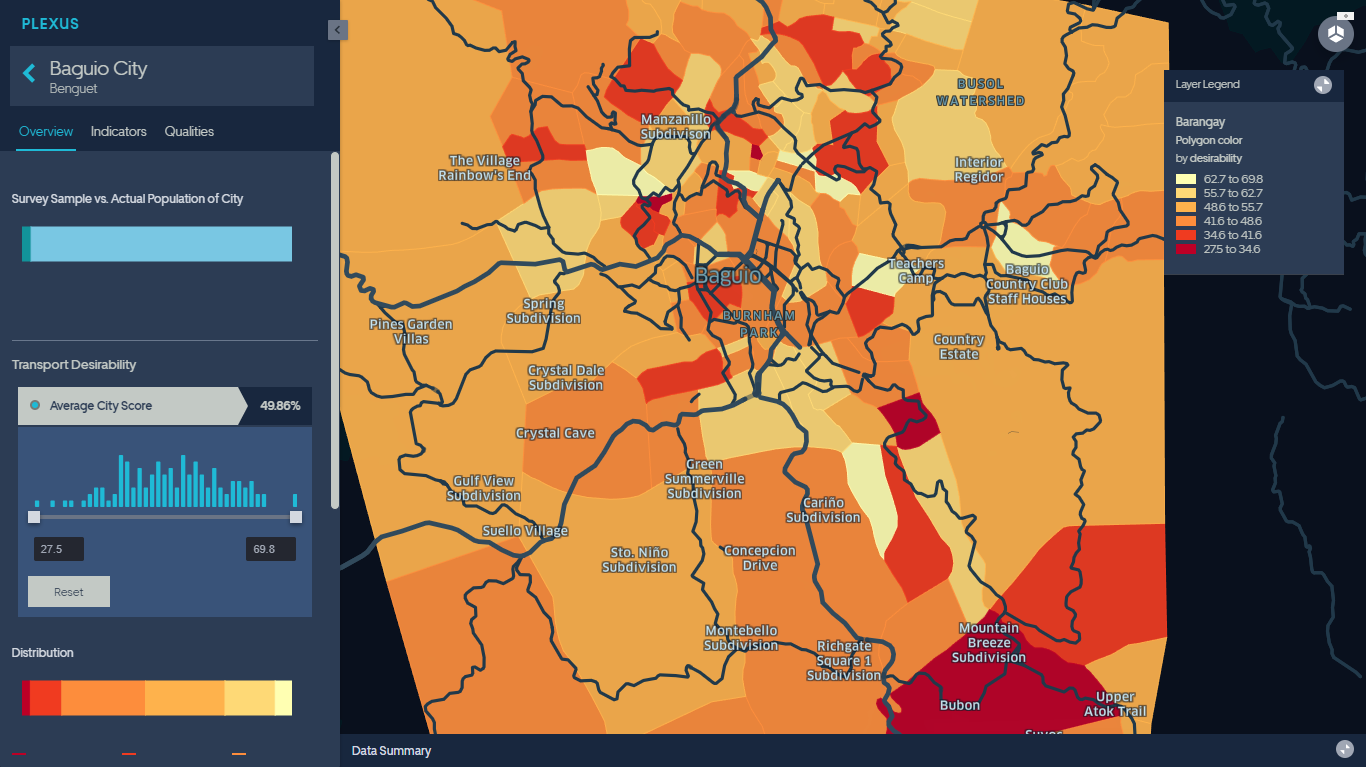
\includegraphics[width=0.9\columnwidth]{figures/overview.PNG}
  \caption{Overview of Plexus showing the overall city information in the left panel, and the choropleth map with its corresponding legend }~\label{fig:KeplerInitialView}
\end{figure}

An initially provided with a list of locations are accessible to the user. Before proceeding to the interactive map, the user may opt to select a location to be presented and assessed. Once a location is selected, the user will be presented with an interactive map and a visible left side panel. The interactive map could be interacted with using elements on the left side panel and interacting with the map itself. The map could be used for visualizing transport desirability-related scores and data.

\subsubsection{Techniques for Visualizing Transport Desirability-related Scores}
Each map view is separated by city based on the user\'s choice and is overlaid by a choropleth map. Participants deemed the choropleth map as the best way to visualize transport desirability scores. 

The map displays the transport desirability score per barangay using a quantize color scale. As seen in Figure \ref{fig:KeplerInitialView}, the color scheme used ranges from light yellow for a high desirability and indicator score, to dark red for a low score. The color scheme initially used ranged from light green to dark blue during UT1. However, it did not help in intuitively determining which areas need transport intervention for users, especially with UT1 novices. Therefore, we made use of red to point out problematic areas for the next implementation. According to 2UN1, \textit{"it\'s obvious that red means danger"}, which was the same sentiment of 89\% of UT2 novices. UT3 and UT4 participants also did not struggle with finding the meaning of red barangays. This change made determining problematic barangays easier to determine for users. 

The legend for the map colors are located in a collapsible panel on the upper right corner of the screen to guide users in interpreting the colors. The order of the colors in the legend were changed when UT1 novices had trouble determining which colors were positive and negative. 1UN3 stated that the reason behind his confusion was \textit{"... the bad color is on the top of the legend, when the legend should be showing the positive color first, like the y-axis [positive numbers found above negative numbers]"}. In the initial stages of the system, the road network of the city was not included in the map view, but was later included since UT1 participants deemed this important \textit{"to be more familiar with the area"}.

\subsubsection{Techniques for Visualizing Other Related Data}
As presented in Figure \ref{fig:KeplerAmenities}, an icon map was used in visualizing amenities found in a city. An icon map was one of the suggested visualizations in the first co-design session to present amenities. Each category for amenities were represented by different icons that are visually descriptive to make the icons discernible. Since we could not add or modify icons, we picked icons that had the nearest relation possible to the amenities. Aside from this, the colors were also initially dependent on the amenity category, but was visually overwhelming for UT1 participants. All UT1 participants states that \textit{"there are too many colors"} when all amenity categories were visible on the map. Although the ideal solution would be to add a circular background or pin to the icons, it could not be implemented. Due to this, all icons were colored white for a work around solution.

\begin{figure}
\centering
  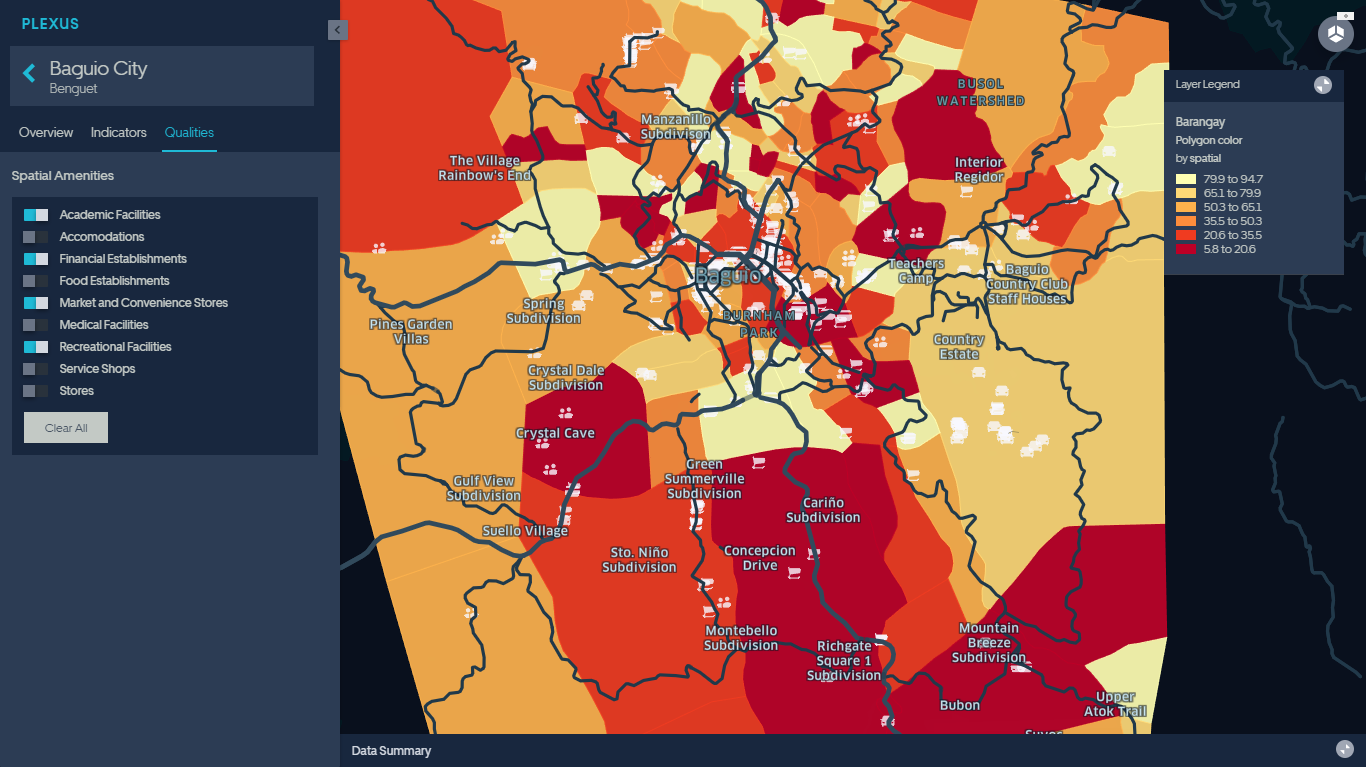
\includegraphics[width=0.9\columnwidth]{figures/kepler9.PNG}
  \caption{Amenities such as academic facilities and recreational facilities are made visible on the map using the left panel}~\label{fig:KeplerAmenities}
\end{figure}

Desire lines, a visualization for origin-destination data and a suggested visualization during the first co-design session, are displayed using a range of blues to contrast the colors in the choropleth map as shown in Figure \ref{fig:KeplerDesireLines}. Desire lines represent the number of people going from a certain origin to a destination, with a darker blue signifying a larger amount of people. The implementation only displays arcs with no visible arrow due to framework limitations. As a result, the frequent origin and destinations of the barangay are shown in the right panel when a barangay is clicked. 

\begin{figure}
\centering
  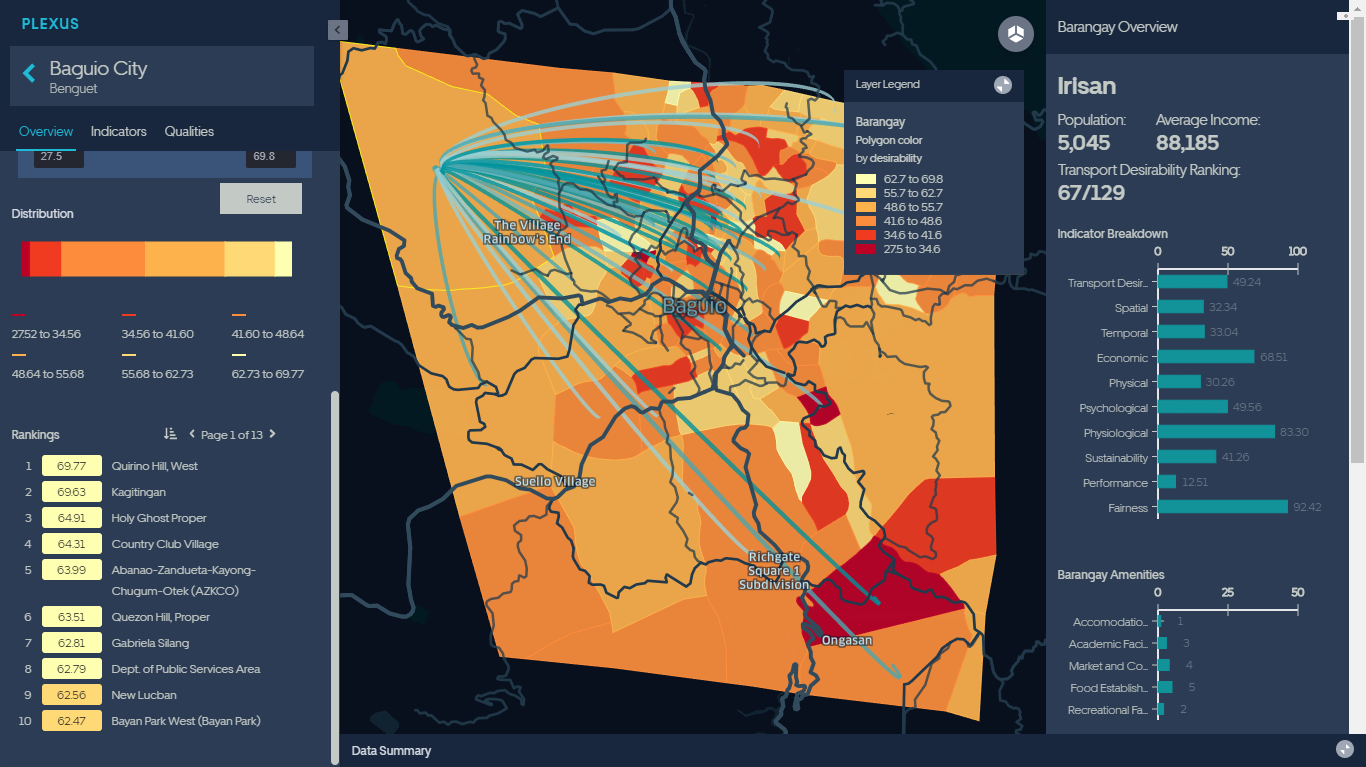
\includegraphics[width=0.9\columnwidth]{figures/overview2.PNG}
  \caption{Desire lines showing the barangay Irisan as the origin, its corresponding destinations, and an overview of the barangay in the right panel }~\label{fig:KeplerDesireLines}
\end{figure}

\subsubsection{Interactivity of Map}
The interactivity of the map allows the user to hover or click on a certain barangay. Once hovered, a tooltip will be shown to display the barangay name and its transport desirability score. When transport desirability-related scores are filtered, barangays that do not meet the criteria of the filter will be left with only their borders.  Lastly, when a barangay on the map has recorded origin-destination data and is clicked, its corresponding origin-destination desire lines will appear. Once a desire line is hovered on, it shows the volume of commuters with that path. Moreover, \textit{"Origin to destination"} was a confusing header for the textbox. 2UN1 stated \textit{"which barangay is the origin? It [the textbox] is confusing since it doesn\'t show the names of the origin and destination."} Overall, 82\% of UT2 participants and 66\% of UT3 participants had the same sentiment. Therefore, this was changed to \textit{"<Origin Barangay name> to <Destination Barangay name>"} for the following test, along with new right panel interactions. 


\subsection{Investigating City and Barangay Data through Side Panels}
Non-geographical data, such as statistical visualization techniques and aggregated datasets, were also utilized in order to describe and give an overview of a city and barangay. Two panels were situated in the left and right sides of the screen with different purposes.

The left side panel holds the city information. The panel has three tabs namely: \textit{Overview}, \textit{Indicators}, and \textit{Qualities}, which is shown in Figure \ref{fig:KeplerInitialView}. The \textit{Overview} tab serves as a general overview of the city which contains the actual and sample population of the city, the ranking of barangays arranged from highest to lowest transport desirability score, the transport desirability score of the city, and the distribution of transport desirability scores within the city. The rankings if the barangays are color-coded similar to the map. Rankings were incorporated as “Rankings are important to help users determine what barangays to focus on”, which was a statement from one of the experts during the second co-design session. Initially, the transport desirability score was included in the \textit{Indicator} tab, but was moved because it is not actually a part of the indicators. Moreover, UT2 Novices could not quickly find the transport desirability score of the city, leading to the decision to move it to the Overview tab. 

The \textit{Indicator} tab shows the indicator scores listed as buttons, with their corresponding score displayed at the right side. Clicking an indicator reflects on the choropleth map and shows a range filter as shown in Figure \ref{fig:KeplerIndicatorActive}. Each indicator was also provided a description and can be accessed by hovering on its corresponding button. Initially, descriptions were brief descriptions of each indicator. However, the descriptions led to multiple misunderstandings of the transport desirability framework. One example was 2UN1, who stated in this analysis that \textit{"desirability is low here because it is a busy area and people can easily walk there. Since terrain could be high and low, it\'s also hard to get good transportation."} He had a misconception that low desirability score meant low availability of transport modes, when in fact transport desirability means the desirability of an area based on accessibility of amenities and transport modes, travel cost and travel time, and the experiences of residents during flooding and using transportation. All UT2 novices had multiple misconceptions. 2UN4 gave an insight that \textit{"the descriptions are helpful, but they leave me with a lot of questions as to what it means."} This led us to further improve the descriptions by adding possible reasons for a low score and what a low score means in layman terms. This was implemented in UT3, wherein all participants did not have misconceptions about transport desirability and its indicators. 

Lastly, the \textit{Qualities} tab contains functions for amenities. A user can toggle the visibility of an amenity category on the map as seen in Figure \ref{fig:KeplerAmenities}.

%!!!!!!!!!!!!!!!!
\begin{figure}
\centering
  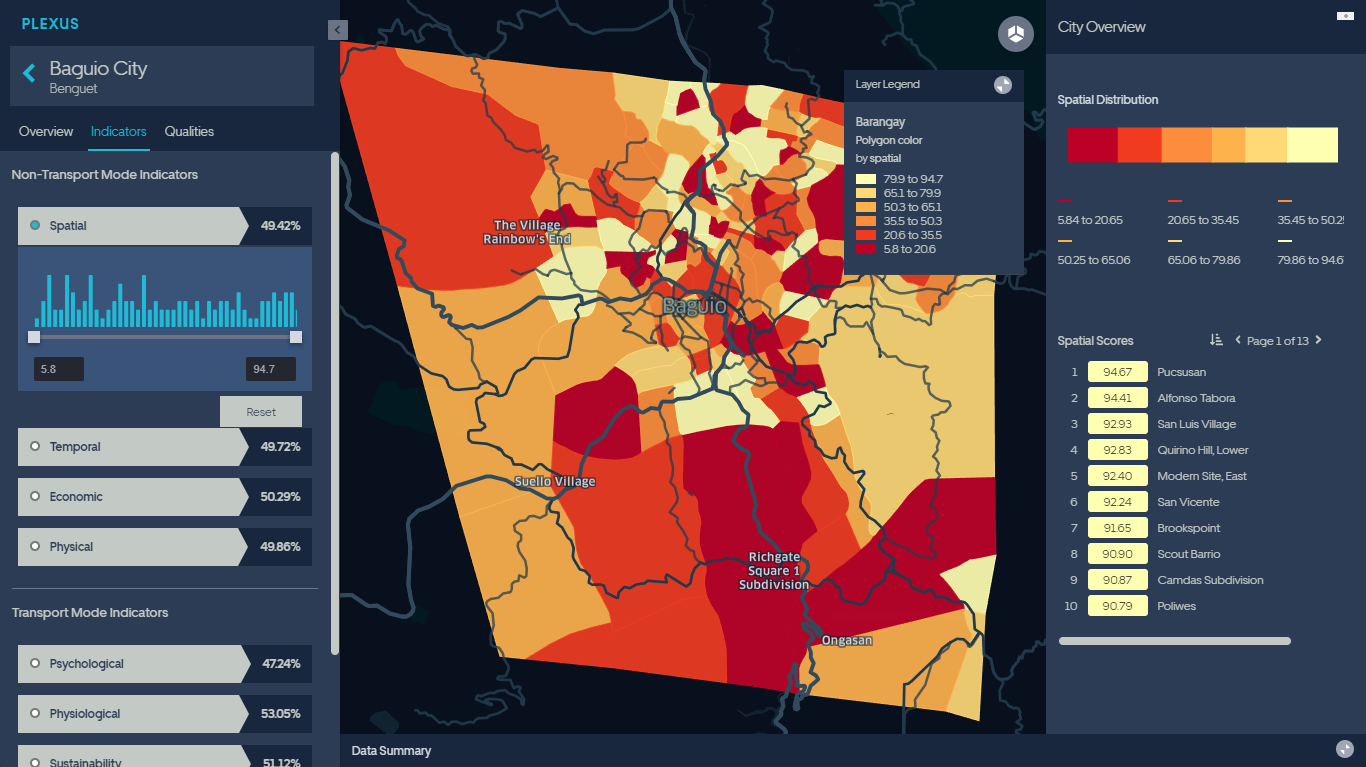
\includegraphics[width=0.9\columnwidth]{figures/indicator.PNG}
  \caption{A distribution and barangay ranking according to the spatial amenity is shown on the right panel}~\label{fig:KeplerIndicatorActive}
\end{figure}

The right panel displays if either an indicator is selected on the right panel or if a barangay is selected on the map. When an indicator is selected, the distribution of the indicator scores in a quantize color scale are presented in a stacked bar chart, and the rankings of all barangays according to the selected indicator are shown, as seen in Figure \ref{fig:KeplerIndicatorActive}. When a barangay is clicked, shown in Figure \ref{fig:KeplerDesireLines} only the barangay information is shown. This was done to segregate the purpose of the panels. The name, population, average income, and the ranking of the barangay according to the selected indicator or transport desirability are positioned at the topmost part of the panel. Aside from this, a bar graph displaying the breakdown of the barangay\'s indicator scores are also positioned in this panel to supply an overview of its current state of transportation. A bar graph was used instead of multiple pie charts for indicators to conserve space and to compare the scores of an indicator to other indicators.


\begin{figure}
\centering
  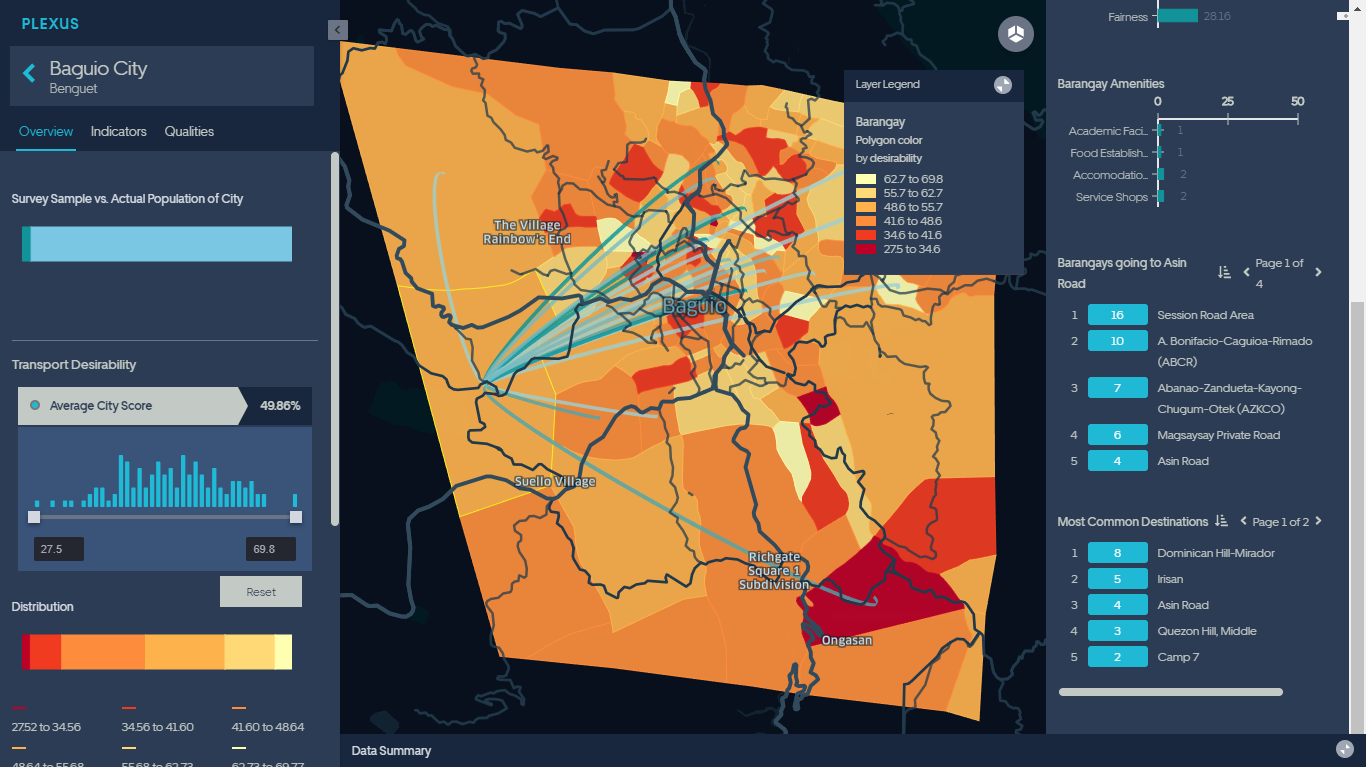
\includegraphics[width=0.9\columnwidth]{figures/overview-barangay-2.PNG}
  \caption{Occurring origins and frequent destination of Asin Road situated in the right panel}~\label{fig:KeplerBarangayContd}
\end{figure}

\subsection{Expert-Authored Data Stories}
The data stories are located in the bottom panel in the screen intends to present a visualized overview of the state of indicators throughout all barangays in the city. From UT2, quality of novice assessments were satisfactory with an average score of 65\%. However, experts highlighted that novices were not maximizing the information available in the system, which was also a main observation during UT2. We further concluded that novices need data stories to guide them during assessment with UT3 and UT4 insights stating that a guide lessens mental workload and boost confidence in novices and the complexity of the transport desirability framework affects novice assessment. Therefore, we collaborated with experts to curate data stories that would guide novices in using the transport desirability framework in assessment. We decided to create separate tabs for city characteristics and city transport desirability report. 

The city characteristics tab consists of an overview of the city\'s amenities, frequent destinations, mode share, demographics, and an interactive way to see all scores of the barangays. This tab aims to gives context to the user before going to the transport desirability report tab. The following section details the components of the tab:


\subsubsection{Parallel Coordinates and Table View of Data}
The parallel coordinates hold the indicators as the items in the x-axis and the barangays as the lines, as illustrated in Figure \ref{fig:KeplerParallelCoords}. These parallel coordinates and tables are more catered to showing trends in the indicator scores and can be used in comparing the scores of multiple barangays at once. During design critiques with experts, parallel coordinates were not a suggested feature to the data story. However, we observed that all UT2 novices frequently used parallel coordinates in their assessments. 2FN2 stated that it is useful because \textit{"it gives an overview of the data without me doing much."} It can be filtered using the transport desirability and indicator range filters in the left panel. The colors used in the parallel coordinates are similar to the colors presented in the choropleth map to immediately form a darker shade in the instance of multiple barangays having the same values or trends. The table will only show the data selected in the parallel coordinates, and all data will be shown if this does not apply. In the table, the columns presented are the barangay name, average income, population, transport desirability score, and their corresponding indicator scores and can be sorted in either ascending or descending order. During UT2 and UT3, most participants were confused with the interactivity of the parallel coordinates. Therefore, we modified the sorting function to be activated through the table column names instead. This came from 2UN6, who stated that \textit{"in the websites that I regularly use, I just click on the column names to sort that column. It makes more sense to me if I can just click on the column name."}

\begin{figure}
\centering
  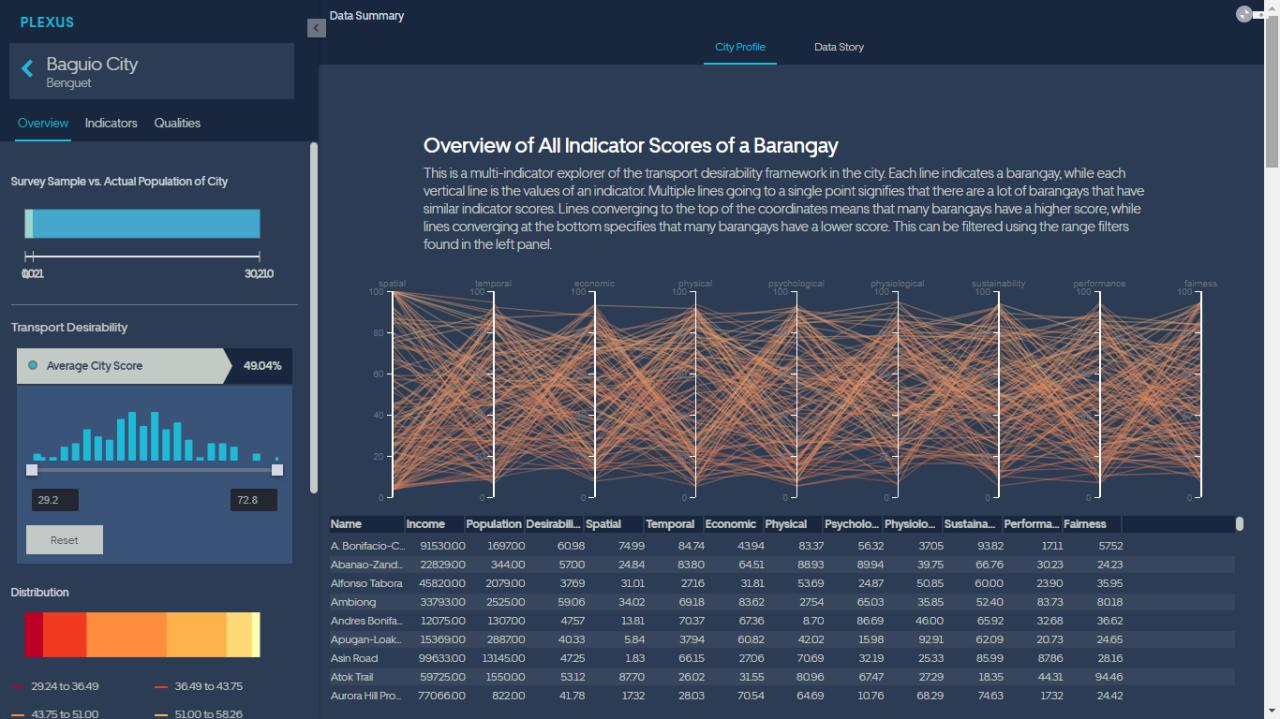
\includegraphics[width=0.9\columnwidth]{figures/latest-screens/pcords.jpg}
  \caption{Parallel coordinates and its corresponding data in table view showing the indicators of the barangays}~\label{fig:KeplerParallelCoords}
\end{figure}


\subsubsection{Comparison of Transport Desirability and Indicator Scores}
As seen in Figure \ref{fig:KeplerScatterPlot}, scatter plots were utilized in order to show a correlation between the transport desirability score and indicator score. This was done to give the user a bi-variate view of data that could help in defining which indicators greatly affect the city\'s overall transport desirability.

\begin{figure}
\centering
  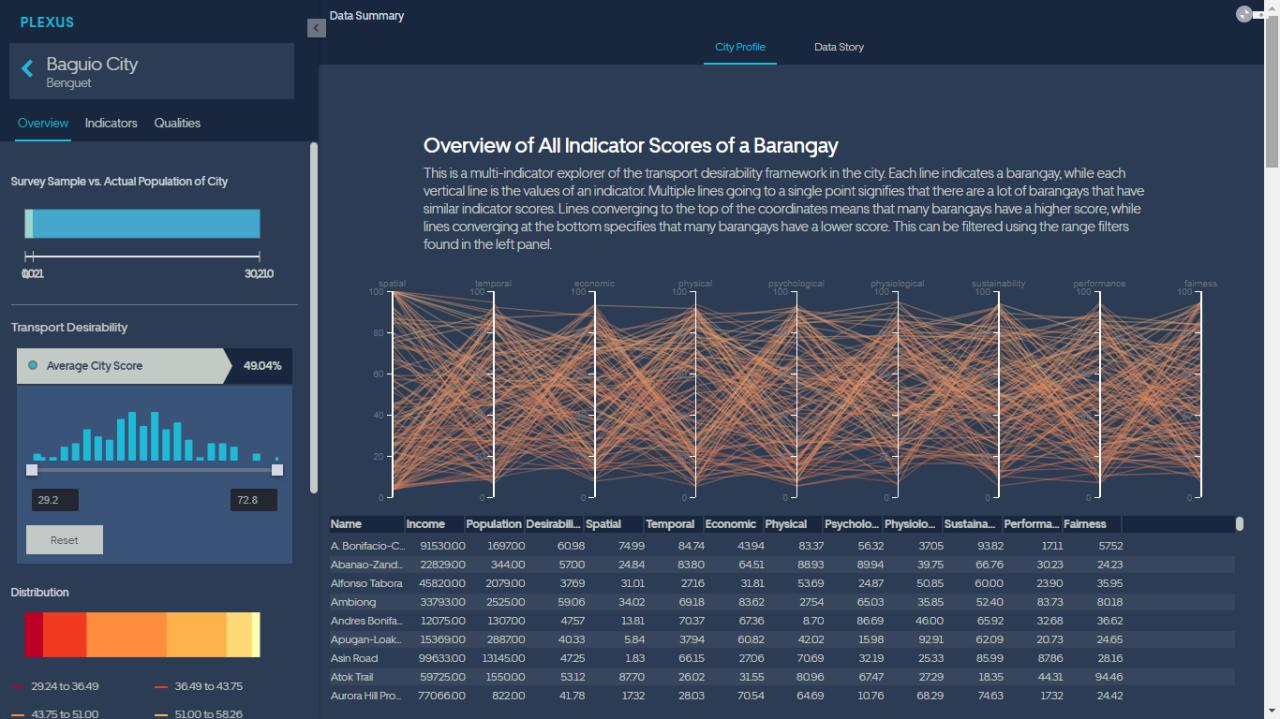
\includegraphics[width=0.9\columnwidth]{figures/latest-screens/pcords.jpg}
  \caption{Scatter plots showing the relationship of all indicators and the transport desirability score}~\label{fig:KeplerScatterPlot}
\end{figure}

\subsubsection{City Amenities}
Both experts from the second co-design session identified amenities as information relevant in all indicators. This is supported by LGU participants in the first co-design session. G2 from the first co-design session stated that location of amenities is the most important information to him because \textit{"traffic is always present near amenities, and it is my job to place amenities in places that won\'t cause traffic."} 

% HI REMOVED THIS KASI WALA NA FREQUENT DESTINATIONS SA FINAL
% Also, G1, G3, and G4, stated that paths that lead to frequent destinations are the focus of most of their policies. 

A summary of city amenities are presented by category and their corresponding count. These information are shown as bar charts as shown in Figure \ref{fig:KeplerAmenitiyModeShare}.


\begin{figure}
\centering
  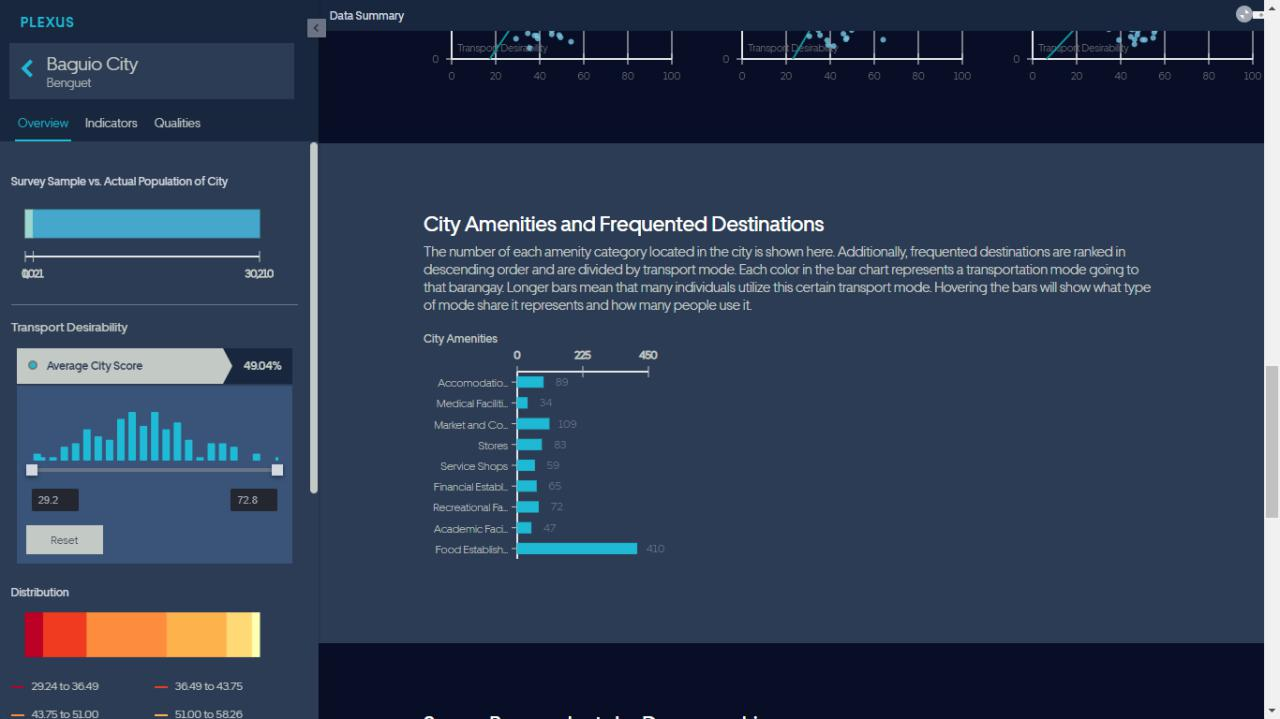
\includegraphics[width=0.9\columnwidth]{figures/latest-screens/amenities.jpg}
  \caption{City amenities bar chart showing the number of amenities per category, and the frequent destinations bar chart showing the list of frequented barangays partitioned by mode share}~\label{fig:KeplerAmenitiyModeShare}
\end{figure}

\subsubsection{Mode Share by Demographic}
The mode share and demographics from the sample population that was surveyed can be classified by sex, income level, and age. Based from the second co-design, both mode share and demographics were the most important information to know before proceeding to transport desirability assessment. These are then separated by barangay, and can be helpful in canvassing factors that could have an effect in transportation behavior. These factors are represented through a stacked bar chart to see its distribution in both the city and the barangay. This can be seen in Figure \ref{fig:KeplerSurveyShare}.

\begin{figure}
\centering
  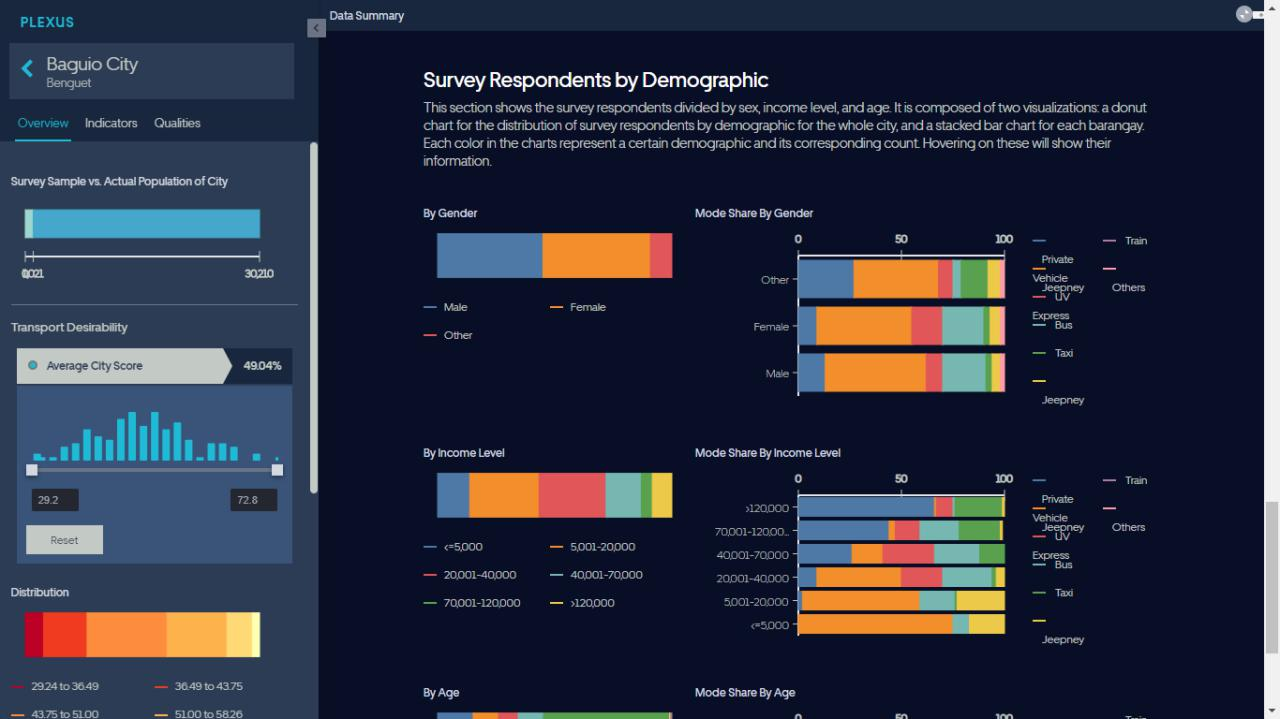
\includegraphics[width=0.9\columnwidth]{figures/latest-screens/modeshare.jpg}
  \caption{Visualization of mode share and demographics in the city organized by sex, income level, and age}~\label{fig:KeplerSurveyShare}
\end{figure}

The transport desirability report tab aims to guide users on how to use transport desirability in their assessment. A transport desirability expert was consulted in formulating the flow of the data story. According to the expert, \textit{"the [ideal] top of mind question [of a user] is \'is the city okay? What are the positive features and negative features of the city?\'. With that, I think the analysis should be top-down."} Therefore, we decided to have an Overview section that shows the state of the city\'s transport desirability and a Diagnosis section that breaks down important indicators through explanatory data and narratives.

\subsubsection{City Profile section}
\begin{figure}
\centering
  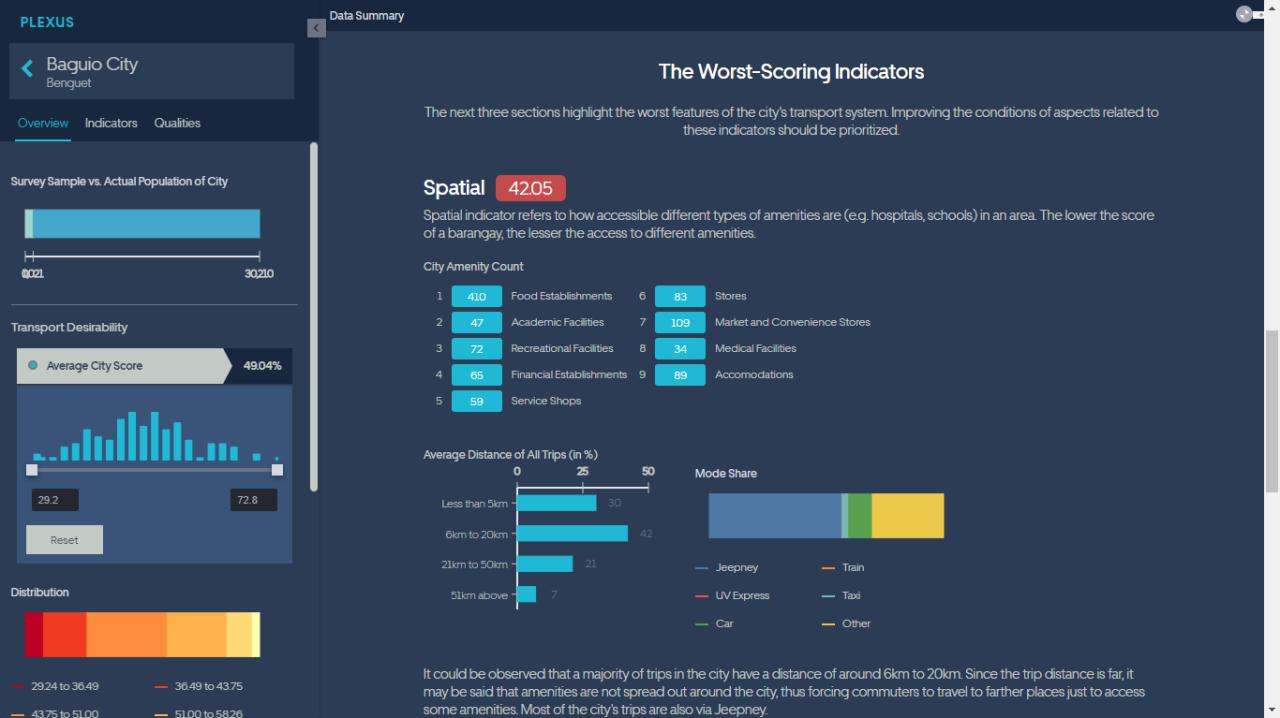
\includegraphics[width=0.9\columnwidth]{figures/latest-screens/city-1.jpg}
  \caption{Transport indicators of the city listed from best to worst}~\label{fig:CityProf}
\end{figure}

The City Profile section shows the city\'s score and its rank among other cities as seen in Figure \ref{fig:CityProf} These were suggested by not only the transport desirability expert, but also UT2 and UT3 LGU participants. 2FN2 gave insights to this suggestion by declaring \textit{"I want to know how the other cities are doing so I can follow or take inspiration from some of their policies."} Additionally, a ranking of the city\'s indicators was added to the section to quickly inform the user of the positive and negative aspects of the city\'s transport desirability. To help the user in formulating an overview of the city, it also lists the top and bottom indicators in the city, as well as the factors that affect them.
% ADD MORE INFORMATION ONCE EXPERIMENT IS DONE

\subsubsection{Diagnosis section}
\begin{figure}
\centering
  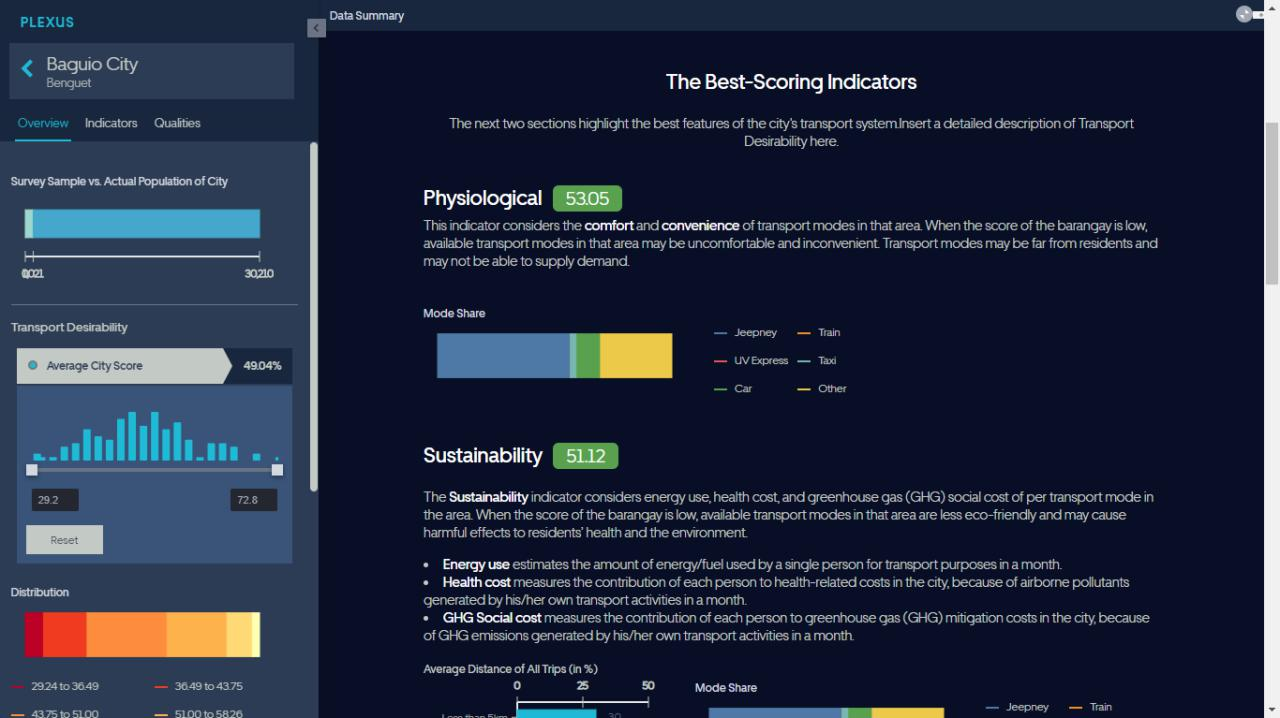
\includegraphics[width=0.9\columnwidth]{figures/latest-screens/city-2.jpg}
  \caption{The top 2 indicators for the city, with its corresponding qualities}~\label{fig:Diagnosis}
\end{figure}

\begin{figure}
\centering
  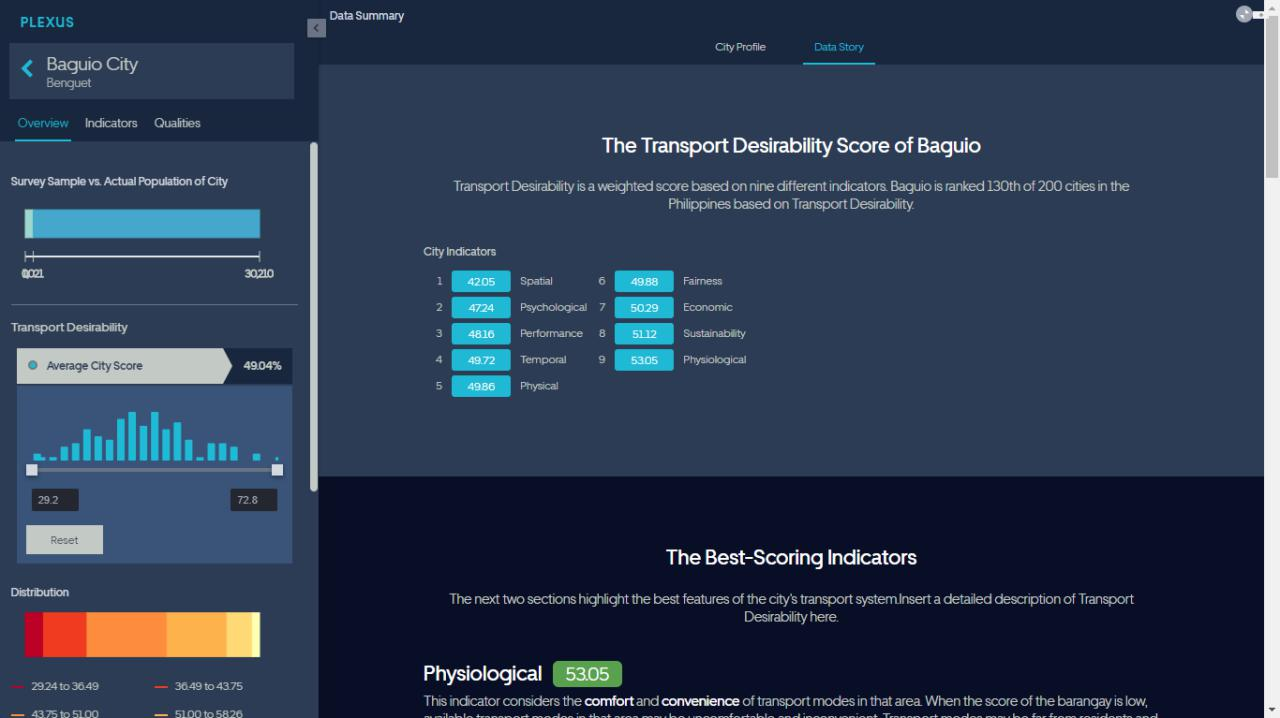
\includegraphics[width=0.9\columnwidth]{figures/latest-screens/city-3.jpg}
  \caption{The bottom 3 indicators for the city, information regarding why the scores are as is}~\label{fig:Diagnosis2}
\end{figure}

As seen in Figure \ref{fig:Diagnosis}, the top two indicators with the highest scores are presented first to the user. According to the expert, showing positive aspects first will \textit{"... engage users and be more open to learn about the negative aspects."} Depending on the indicator, reasons behind the high score are shown through data visualizations. Each indicator is accompanied with a narrative of the reasons behind the high score and suggested recommendations to improve the score. After the top two indicators with the highest scores, the top three lowest scores are presented since \textit{"the lowest scores are more relevant for the user since he will use these to create policies or other possible solutions."} Just like the previous indicators, each lowest indicator is accompanied with explanatory data and a narrative, which can be seen as Figure \ref{fig:Diagnosis2}. 
% ADD MORE INFORMATION ONCE EXPERIMENT IS DONE

\section{Experimental Design}
For the experiment that was conducted, twelve novices created transport desirability assessments based on given tasks. However, these novices were divided into three groups; Each group utilized a different tool for their assessment. The first group utilized spreadsheet applications since some LGU officials that we have consulted with currently use these to assess information. The other two groups utilized Plexus, but were divided into those who used it with and without data stories. After each task, each participant answered a NASA-TLX questionnaire to quantify the mental workload endured for each task. Moreover, each participant was asked about their experience doing the task to qualitatively determine the system\'s usability. For result analysis, the ratings will be on a scale of 1 to 7, with 7 being excellent and 1 being highly unsatisfactory. The NASA-TLX results will be used to compare the different groups and to check if data stories positively affected the quality of assessments. The average raw ratings of the participants per subscale were computed as the overall average subscale score per group.

% % BAKA DI NA GAWIN
% % For result analysis, experts in transport desirability assessment will be rating the resulting assessments of novices depending on their process and their output. The ratings will be on a scale of 1 to 7, with 7 being excellent and 1 being highly unsatisfactory. Both expert ratings and NASA-TLX results will be used to compare the different groups and to check if data stories positively affected the quality of assessments.  

\section{Discussion}

\begin{table}[]
\toprule
\small
\begin{tabular}{lrrrrr}
{\small\textit{Subscale}}
& {\small \textit{Task 1}}
& {\small \textit{Task 2}}
& {\small \textit{Task 3}} 
& {\small \textit{Task 4}}
& {\small \textit{Average}} \\
\midrule
\multicolumn{6}{c}{Spreadsheet Applications}                 \\
\midrule
Mental Demand   & 65.00     & 57.50   & 72.50 & 70.00  & \cellcolor[rgb]{0.78,0.78,0.78} 66.25  \\
Physical Demand & 30.00     & 37.50   & 33.75  & 35.00   & 34.06 \\
Temporal Demand & 63.75  & 41.25  & 62.50   & 55.00     & 55.63  \\
Performance     & 53.75  & 90.00     & 51.25  & 48.75  & 60.94 \\
Effort          & 53.75  & 56.25  & 68.75  & 70.00     & 62.19 \\
Frustration     & 53.75  & 45.00     & 77.50   & 70.00   & 61.56 \\
\midrule
\multicolumn{6}{c}{Plexus without Data Stories}                      \\
\midrule
Mental Demand   & 50.00  & 56.25  & 57.50  & 52.50  & \cellcolor[rgb]{0.78,0.78,0.78} 54.06   \\
Physical Demand & 30.00  & 25.00  & 20.00  & 31.25  & 26.56   \\
Temporal Demand & 30.00  & 35.00  & 18.75  & 38.75  & 30.63   \\
Performance     & 50.00  & 57.50  & 76.25  & 40.00  & \cellcolor[rgb]{0.78,0.78,0.78} 55.94   \\
Effort          & 40.00  & 53.75  & 37.50  & 45.00  & 44.06   \\
Frustration     & 40.00  & 30.00  & 23.75  & 40.00  & \cellcolor[rgb]{0.78,0.78,0.78} 33.44   \\
\midrule
\multicolumn{6}{c}{Plexus with Data Stories}                         \\
\midrule
Mental Demand   & 53.75  & 41.25  & 57.50  & 45.00 & 49.38  \\
Physical Demand & 27.50   & 35.00     & 41.25  & 40.00  & 35.94 \\
Temporal Demand & 35.00     & 36.25  & 41.25  & 37.50 & 37.50    \\
Performance     & 65.00     & 57.5   & 58.75  & 61.25  & \cellcolor[rgb]{0.78,0.78,0.78} 60.63  \\
Effort          & 45.00     & 41.25  & 56.25  & 53.75  & 49.06 \\
Frustration     & 40.00     & 28.75  & 43.75  & 37.50   & 37.50   
\end{tabular}
\bottomrule
\caption{Average values of NASA-TLX subscales per task and tool used with notable values highlighted}~\label{tab:tlx}
\end{table}

Through the co-design approach, we were able to identify that the mental models of novices and experts were different. Novices use trial-and-error to find solutions to problems since they have limited access to resources and data. In terms of their planning and assessment process, they implement a bottom-up approach, wherein they identify major problems through collating their observations. They mainly use travel count and location of amenities to help in their decision-making. If provided with other data, they may have difficulty using these to create conclusions. During the first co-design session, novices only suggested map-related visualizations, which are visualizations that mainly use for zoning. In the usability tests, it was evident that novices needed more time to understand the interactions and visualizations in the tool. Novices also had difficulty using multiple data to conclude indicator scores without a guide. Hence, data stories were useful for novices to understand concepts and connect data presented to create conclusions. 

On the other hand, experts are knowledgeable in using transport planning systems, which allowed them to be more open to different visualizations and interactions. This was evident during usability tests as experts were immediately comfortable with using the tool. They use a top-down approach when planning and assessing, and they highly depend on travel demand and mode share information. According to transport desirability experts, the ideal process of transport assessment is a top-down approach. More than travel demand and amenities, these experts want users to use other data related to commuter experience when creating assessments. Insights from both types of users were essential in implementing ths system.

Co-design sessions, design critiques, and task-based tests were effective in refining features, visualizations, and interactions in the tool. Co-design sessions gave a skeleton to create prototypes, design critiques during the usability tests resulted to specific comments and suggestions for refinement, and task-based usability tests effectively presented the confidence and mental workload of participants per task to give insights on the complexity and intuitiveness of the tool. However, these activities could be improved in terms of methods and participants. During the first co-design, having provincial LGUs and more transport engineering experts could have led to more diverse results, which could have lessened new suggestions during UT3 and UT4. Novices were abstracted from transport desirability experts due to conflicting schedules. This abstraction may have had an effect on the data and interface suggestions, as novices were not able to comment on the suggestions\' complexity. Another co-design session with transport desirability experts and novices should have been conducted for experts to understand the mental models of novices as well. Moreover, only UT2 had experts rate the quality of novice assessments. UT3 could have had experts rate as well to determine the effect on quality after utilizing new descriptions on unfamiliar users.

% commented out kasi baka mahaba na discussion :-(
% When designing a multi-panel novice support tool, a maximum of two panels can only be shown to users. This was an insight during UT1 when all users were overwhelmed by having 3 panels open at a time. Additionally, although experts identified the parallel coordinates as a visualization that could be removed from the tool, it was frequently used by novices in all usability tests, and could be an effective alternative to bivariate maps. Moreover, superimposing bar graphs or pie charts to maps would be confusing for novices; Panels containing these visualizations could be a better alternative.

Initially, we implemented the system to focus more on the interactivity. However, users were looking for explicit information to guide their conclusions. This led to major changes beginning in UT2; The tool had more data visualizations related to the indicators and a data story panel presenting city characteristics, which resulted to novices being more confident with their assessments. Although data stories and related data were effective, quality of assessments could still be improved. From UT3 and UT4, we concluded that novices may not fully understand transport desirability while using the tool. Therefore, we decided to make a narrative data story showing the ideal flow and use of available data when doing transport desirability assessment. Modified visualizations and features were then present in the last testing.

% UT3 STUFF, CAN BE MOVED (START)
From the experimental design, we found that those who used spreadsheet applications were slower in making assessments as compared to using Plexus. The users mentioned that they would want to do the tasks as fast as possible, and wished to see lesser numbers and raw figures. Additionally, they also wanted the option to visualize roads and amenities. After their tasks, they were shown the system. Based on the NASA-TLX evaluation, we noted that the heaviest subscales that contribute to their mental workload were mental demand, frustration, and effort. All participants who used spreadsheets were shown the system with data stories. Overall, they would have preferred to use the system instead since using spreadsheet applications was difficult. A participant stated that \textit{"there are so many numbers [in the spreadsheet], all I want to do is look away and do assessments as fast as possible. But with the tool, it engages me and all the information is presented visually."} Participants who utilized Plexus with no data stories found the tasks easy, with lower mental workload scores compared to the previous group. However, the resulting assessments were only based on the descriptions of the indicators in the left panel and their assumptions since they were observed to cite information that were not found in the system. The mental demand is higher than utilizing data stories since participants have a difficulty in understanding information presented to them.  We also observed that there were misunderstandings about the indicators due to the descriptions being brief. Due to this, participants who used the tool without data stories had the lowest performance score out of the three groups and were less satisfied with their assessments. 

Lastly, for those who utilized Plexus with data stories, it was observed that they were the fastest in making assessments. Aside from these, their assessments are relatively more in-depth, and they tend to use the system more as compared to the participants making some assumptions without the data stories. They also extensively used the data stories component, particularly the discussion about the city's top and bottom indicators, when assessing the city as a whole. Since the indicators had additional information framed as narratives, the participants were able to understand the framework better than those who relied on the descriptions alone and obtained the lowest average mental demand score. In terms of performance, the group obtained a score similar to the group that utilized spreadsheets but experienced less difficulty in creating assessments. All participants mentioned that the tasks were easy and would be harder to do without the data stories because they would have had to look at all barangay characterisitcs to reach a city assessment. 

% UT3 STUFF, CAN BE MOVED (END)

\section{Conclusion and Future Work}
When designing a transport-related novice support tool for assessment, interactivity must be balanced with data stories for users to have less mental workload and more confidence when using the tool. Data stories ensure that novices understand the ideal flow of processes. Additionally, narratives and descriptions in layman terms clarifies complex concepts and processes. Although experts are open to use multiple visualizations and interactions, novices were more inclined to use familiar visualizations. Parallel coordinates and panels are good alternatives to bivariate maps and superimposed visualizations on maps, as novices were keen to utilize these visualizations for their assessments. Road networks, boundaries, and landmarks are beneficial additions to maps for users to gain familiarity of the area.  In this study, co-design with both experts and novices ensured that best practices and features were chosen without sacrificing standard practices yet simple for novices. With experts and novices collaborating, they discussed the most important features and visualizations that are helpful for the implementation of a transport assessment tool. 

% \subsection{References and Citations}

% Use a numbered list of references at the end of the article, ordered
% alphabetically by last name of first author, and referenced by numbers
% in
% brackets~\cite{acm_categories,ethics,Klemmer:2002:WSC:503376.503378}.
% Your references should be published materials accessible to the
% public. Internal technical reports may be cited only if they are
% easily accessible (i.e., you provide the address for obtaining the
% report within your citation) and may be obtained by any reader for a
% nominal fee. Proprietary information may not be cited. Private
% communications should be acknowledged in the main text, not referenced
% (e.g., ``[Borriello, personal communication]'').

% References should be in ACM citation format:
% \url{http://acm.org/publications/submissions/latex_style}. This
% includes citations to internet
% resources~\cite{acm_categories,cavender:writing,CHINOSAUR:venue,psy:gangnam}
% according to ACM format, although it is often appropriate to include
% URLs directly in the text, as above.


% % Use a numbered list of references at the end of the article, ordered
% % alphabetically by first author, and referenced by numbers in
% % brackets~\cite{ethics, Klemmer:2002:WSC:503376.503378,
% %   Mather:2000:MUT, Zellweger:2001:FAO:504216.504224}. For papers from
% % conference proceedings, include the title of the paper and an
% % abbreviated name of the conference (e.g., for Interact 2003
% % proceedings, use \textit{Proc. Interact 2003}). Do not include the
% % location of the conference or the exact date; do include the page
% % numbers if available. See the examples of citations at the end of this
% % document. Within this template file, use the \texttt{References} style
% % for the text of your citation.

% % Your references should be published materials accessible to the
% % public.  Internal technical reports may be cited only if they are
% % easily accessible (i.e., you provide the address for obtaining the
% % report within your citation) and may be obtained by any reader for a
% % nominal fee.  Proprietary information may not be cited. Private
% % communications should be acknowledged in the main text, not referenced
% % (e.g., ``[Robertson, personal communication]'').

% \begin{table}
%   \centering
%   \begin{tabular}{l r r r}
%     % \toprule
%     & & \multicolumn{2}{c}{\small{\textbf{Test Conditions}}} \\
%     \cmidrule(r){3-4}
%     {\small\textit{Name}}
%     & {\small \textit{First}}
%       & {\small \textit{Second}}
%     & {\small \textit{Final}} \\
%     \midrule
%     Marsden & 223.0 & 44 & 432,321 \\
%     Nass & 22.2 & 16 & 234,333 \\
%     Borriello & 22.9 & 11 & 93,123 \\
%     Karat & 34.9 & 2200 & 103,322 \\
%     % \bottomrule
%   \end{tabular}
%   \caption{Table captions should be placed below the table. We
%     recommend table lines be 1 point, 25\% black. Minimize use of
%     table grid lines.}~\label{tab:table1}
% \end{table}

% \section{Sections}

% The heading of a section should be in Helvetica or Arial 9-point bold,
% all in capitals. Sections should \textit{not} be numbered.

% \subsection{Subsections}

% Headings of subsections should be in Helvetica or Arial 9-point bold
% with initial letters capitalized.  For sub-sections and
% sub-subsections, a word like \emph{the} or \emph{of} is not
% capitalized unless it is the first word of the heading.

% \subsubsection{Sub-subsections}

% Headings for sub-subsections should be in Helvetica or Arial 9-point
% italic with initial letters capitalized.  Standard
% \texttt{{\textbackslash}section}, \texttt{{\textbackslash}subsection},
% and \texttt{{\textbackslash}subsubsection} commands will work fine in
% this template.

% \section{Figures/Captions}

% Place figures and tables at the top or bottom of the appropriate
% column or columns, on the same page as the relevant text (see
% Figure~\ref{fig:figure1}). A figure or table may extend across both
% columns to a maximum width of 17.78 cm (7 in.).

% \begin{figure*}
%   \centering
%   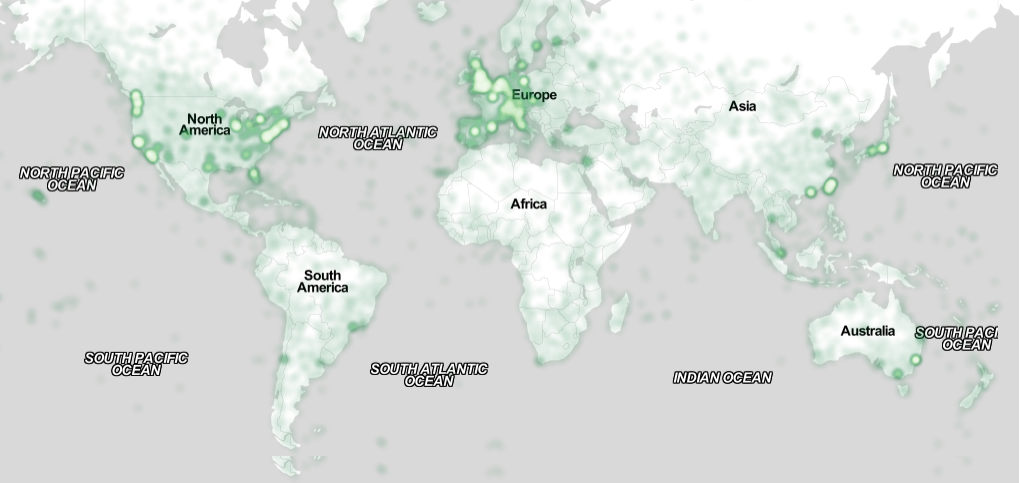
\includegraphics[width=1.75\columnwidth]{figures/map}
%   \caption{In this image, the map maximizes use of space. You can make
%     figures as wide as you need, up to a maximum of the full width of
%     both columns. Note that \LaTeX\ tends to render large figures on a
%     dedicated page. Image: \ccbynd~ayman on
%     Flickr.}~\label{fig:figure2}
% \end{figure*}

% Captions should be Times New Roman or Times Roman 9-point bold.  They
% should be numbered (e.g., ``Table~\ref{tab:table1}'' or
% ``Figure~\ref{fig:figure1}''), centered (if one line) otherwise justified, and placed beneath the figure
% or table.  Please note that the words ``Figure'' and ``Table'' should
% be spelled out (e.g., ``Figure'' rather than ``Fig.'') wherever they
% occur. Figures, like Figure~\ref{fig:figure2}, may span columns and
% all figures should also include alt text for improved accessibility.
% Papers and notes may use color figures, which are included in the page
% limit; the figures must be usable when printed in black-and-white in
% the proceedings.

% The paper may be accompanied by a short video figure (we recommend staying within five
% minutes in length). However, the paper should stand on its own without
% the video figure, as the video may not be available to everyone who
% reads the paper.  

% \subsection{Inserting Images}
% When possible, include a vector formatted graphic (i.e. PDF or EPS).
% When including bitmaps,  use an image editing tool to resize the image
% at the appropriate printing resolution (usually 300 dpi).

% \section{Quotations}
% Quotations may be italicized when \textit{``placed inline''}.

% \begin{quote}
% Longer quotes, when placed in their own paragraph, need not be
% italicized or in quotation marks when indented.  
% \end{quote}

% \section{Language, Style, and Content}

% The written and spoken language of SIGCHI is English. Spelling and
% punctuation may use any dialect of English (e.g., British, Canadian,
% US, etc.) provided this is done consis- tently. Hyphenation is
% optional. To ensure suitability for an international audience, please
% pay attention to the following:

% \begin{itemize}
% \item Write in a straightforward style.
% \item Try to avoid long or complex sentence structures.
% \item Use common and basic vocabulary (e.g., use the word ``unusual'' rather than the word ``arcane''.
% \item Briefly define or explain all technical terms that may be
%   unfamiliar to readers.
% \item Explain all acronyms the first time they are used in your
%   text---e.g., ``Digital Signal Processing (DSP)''.
% \item Explain local references (e.g., not everyone knows all city
%   names in a particular country).
% \item Explain ``insider'' comments. Ensure that your whole audience
%   understands any reference whose meaning you do not describe (e.g.,
%   do not assume that everyone has used a Macintosh or a particular
%   application).
% \item Explain colloquial language and puns. Understanding phrases like
%   ``red herring'' may require a local knowledge of English.  Humor and
%   irony are difficult to translate.
% \item Use unambiguous forms for culturally localized concepts, such as
%   times, dates, currencies, and numbers (e.g., ``1--5--97'' or
%   ``5/1/97'' may mean 5 January or 1 May, and ``seven o'clock'' may
%   mean 7:00 am or 19:00). For currencies, indicate equivalences:
%   ``Participants were paid {\fontfamily{txr}\selectfont \textwon}
%   25,000, or roughly US \$22.''
% \item Be careful with the use of gender-specific pronouns (he, she)
%   and other gendered words (chairman, manpower, man-months). Use
%   inclusive language that is gender-neutral (e.g., she or he, they,
%   s/he, chair, staff, staff-hours, person-years). See the
%   \textit{Guidelines for Bias-Free Writing} for further advice and
%   examples regarding gender and other personal
%   attributes~\cite{Schwartz:1995:GBF}. Be particularly aware of
%   considerations around writing about people with disabilities.
% \item If possible, use the full (extended) alphabetic character set
%   for names of persons, institutions, and places (e.g.,
%   Gr{\o}nb{\ae}k, Lafreni\'ere, S\'anchez, Nguy{\~{\^{e}}}n,
%   Universit{\"a}t, Wei{\ss}enbach, Z{\"u}llighoven, \r{A}rhus, etc.).
%   These characters are already included in most versions and variants
%   of Times, Helvetica, and Arial fonts.
% \end{itemize}

% \section{Accessibility}
% The Executive Council of SIGCHI has committed to making SIGCHI
% conferences more inclusive for researchers, practitioners, and
% educators with disabilities. As a part of this goal, the all authors
% are asked to work on improving the accessibility of their
% submissions. Specifically, we encourage authors to carry out the
% following five steps:
% \begin{enumerate}
% \item Add alternative text to all figures
% \item Mark table headings
% \item Add tags to the PDF
% \item Verify the default language
% \item Set the tab order to ``Use Document Structure''
% \end{enumerate}
% For more information and links to instructions and resources, please
% see: \url{http://chi2016.acm.org/accessibility}.  The
% \texttt{{\textbackslash}hyperref} package allows you to create well tagged PDF files,
% please see the preamble of this template for an example.

% \section{Page Numbering, Headers and Footers}
% Your final submission should not contain footer or header information
% at the top or bottom of each page. Specifically, your final submission
% should not include page numbers. Initial submissions may include page
% numbers, but these must be removed for camera-ready. Page numbers will
% be added to the PDF when the proceedings are assembled.

% \section{Producing and Testing PDF Files}

% We recommend that you produce a PDF version of your submission well
% before the final deadline.  Your PDF file must be ACM DL
% Compliant. The requirements for an ACM Compliant PDF are available at:
% {\url{http://www.scomminc.com/pp/acmsig/ACM-DL-pdfs-requirements.htm}}.

% Test your PDF file by viewing or printing it with the same software we
% will use when we receive it, Adobe Acrobat Reader Version 10. This is
% widely available at no cost. Note that most
% reviewers will use a North American/European version of Acrobat
% reader, so please check your PDF accordingly.

% \section{Conclusion}

% It is important that you write for the SIGCHI audience. Please read
% previous years' proceedings to understand the writing style and
% conventions that successful authors have used. It is particularly
% important that you state clearly what you have done, not merely what
% you plan to do, and explain how your work is different from previously
% published work, i.e., the unique contribution that your work makes to
% the field. Please consider what the reader will learn from your
% submission, and how they will find your work useful. If you write with
% these questions in mind, your work is more likely to be successful,
% both in being accepted into the conference, and in influencing the
% work of our field.

\section{Acknowledgments}

%The authors Ms. Courtney Ngo and Ms. Jennifer Ureta, for offering their guidance and constructive comments that would help in improving the study. The authors would also like to thank the Commission on Higher Education (CHED) for the overall support in performing this study. Furthermore, they would also like to extend their gratitude to the principal investigator of the project, Dr. Jose Bienvenido Manuel Biona, as well as the co-investigators , Dr. Neil Stephen Lopez and Dr. Alexis Fillone, for sharing their expertise with regards to the field of transport desirability. Lastly, the authors 
We would like to thank the participants in the usability testings for giving us fruitful insights that greatly helped in the objective of the study. This research was conducted with funding support from the Commission on Higher Education Grants-in-Aid program of the Philippines under Res. No. 873-2017. Furthermore, we would also like to extend their gratitude to the principal investigator of the project, Dr. Jose Bienvenido Manuel Biona, as well as the co-investigators , Dr. Neil Stephen Lopez and Dr. Alexis Fillone, for sharing their expertise with regards to the field of transport desirability.

% Balancing columns in a ref list is a bit of a pain because you
% either use a hack like flushend or balance, or manually insert
% a column break.  http://www.tex.ac.uk/cgi-bin/texfaq2html?label=balance
% multicols doesn't work because we're already in two-column mode,
% and flushend isn't awesome, so I choose balance.  See this
% for more info: http://cs.brown.edu/system/software/latex/doc/balance.pdf
%
% Note that in a perfect world balance wants to be in the first
% column of the last page.
%
% If balance doesn't work for you, you can remove that and
% hard-code a column break into the bbl file right before you
% submit:
%
% http://stackoverflow.com/questions/2149854/how-to-manually-equalize-columns-
% in-an-ieee-paper-if-using-bibtex
%
% Or, just remove \balance and give up on balancing the last page.
%
\balance{}

% \section{References Format}
% Your references should be published materials accessible to the
% public. Internal technical reports may be cited only if they are
% easily accessible and may be obtained by any reader for a nominal
% fee. Proprietary information may not be cited. Private communications
% should be acknowledged in the main text, not referenced (e.g.,
% [Golovchinsky, personal communication]). References must be the same
% font size as other body text. References should be in alphabetical
% order by last name of first author. Use a numbered list of references
% at the end of the article, ordered alphabetically by last name of
% first author, and referenced by numbers in brackets. For papers from
% conference proceedings, include the title of the paper and the name of
% the conference. Do not include the location of the conference or the
% exact date; do include the page numbers if available. 

% References should be in ACM citation format:
% \url{http://www.acm.org/publications/submissions/latex_style}.  This
% includes citations to Internet
% resources~\cite{CHINOSAUR:venue,cavender:writing,psy:gangnam}
% according to ACM format, although it is often appropriate to include
% URLs directly in the text, as above. Example reference formatting for
% individual journal articles~\cite{ethics}, articles in conference
% proceedings~\cite{Klemmer:2002:WSC:503376.503378},
% books~\cite{Schwartz:1995:GBF}, theses~\cite{sutherland:sketchpad},
% book chapters~\cite{winner:politics}, an entire journal
% issue~\cite{kaye:puc},
% websites~\cite{acm_categories,cavender:writing},
% tweets~\cite{CHINOSAUR:venue}, patents~\cite{heilig:sensorama}, 
% games~\cite{supermetroid:snes}, and
% online videos~\cite{psy:gangnam} is given here.  See the examples of
% citations at the end of this document and in the accompanying
% \texttt{BibTeX} document. This formatting is a edited version of the
% format automatically generated by the ACM Digital Library
% (\url{http://dl.acm.org}) as ``ACM Ref.'' DOI and/or URL links are
% optional but encouraged as are full first names. Note that the
% Hyperlink style used throughout this document uses blue links;
% however, URLs in the references section may optionally appear in
% black.

% BALANCE COLUMNS
\balance{}

% REFERENCES FORMAT
% References must be the same font size as other body text.
\bibliographystyle{SIGCHI-Reference-Format}
\bibliography{sample}

\end{document}

%%% Local Variables:
%%% mode: latex
%%% TeX-master: t
%%% End:
